\documentclass{theme-2614084}
\usepackage{hyperref}
\usepackage{bookmark}
\usepackage{minted}

\usepackage{hyperref}

% =============================================
% Part 0 信息
% =============================================

\mathsetup{
  % 学生姓名
  student-name = {某同学},
  % 学号
  student-id = {2021xxxx},
  % 院系
  department = {电子与信息工程学院},
  % 专业
  experiment = {实验二 MOS管特性和CMOS反相器特性仿真分析},
  % 专业年级
  major = {集成电路设计与集成系统},
  % 日期
  % date = {\today},
}

\begin{document}

% =============================================
% Part 1  封面
% =============================================

\makecover

% =============================================
% Part 2 主文档
% =============================================

\section{实验目的}

MOS管I-V特性和CMOS反相器特性(DC\&TRAN)仿真分析

\begin{enumerate}
  \item 熟悉 Cadence 启动环境
  \item 理解 Analog Environment 启动及仿真信号源和 CSMC 模型库的设置
  \item 掌握运用 Cadence Composer 进行原理图编辑与设计的方法
  \item 掌握运用 Cadence 仿真工具进行电路仿真分析的方法(直流、交流、瞬态分析),深入理解 MOS 管和反相器工作原理
\end{enumerate}

\section{实验环境}

\begin{enumerate}
  \item 硬件: PC 机、服务器
  \item 环境:Unix 操作系统、Cadence 集成电路设计软件
\end{enumerate}

\section{实验内容与步骤}

% (注:按照内容,有截图和说明)

\subsection{实验内容}

\begin{enumerate}
  \item NMOS管的ID-VDS 的仿真(华润上华CSMC0.6um模型库),得到特性曲线(完成任务1、任务2)
  \item CMOS反相器的直流(DC)仿真分析(台积电TSMC0.35um模型库)(完成任务3)。
  \item CMOS反相器的瞬态特性(Tran)仿真分析(中芯国际SMIC 0.18um模型库)(完成任务3)。
\end{enumerate}

\subsection{任务1}

1、在自己目录 \texttt{stuXXX/123} 下启动Cadence  
2、新建 library 为 lab2,新建 file 为 NMOS\_SIM

为本次实验建立模型库

\begin{figure}[H]
  \centering
  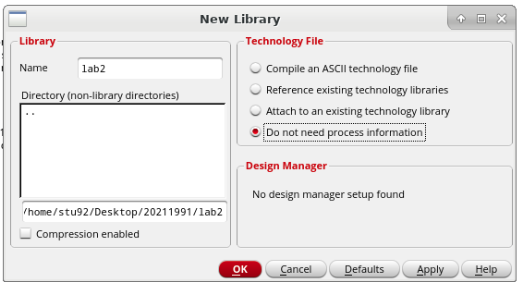
\includegraphics[width=0.8\textwidth]{task1/task1-create-new-library.png}
  \caption{create new Library}
\end{figure}

Draw NMOS\_SIM

\begin{figure}[H]
  \centering
  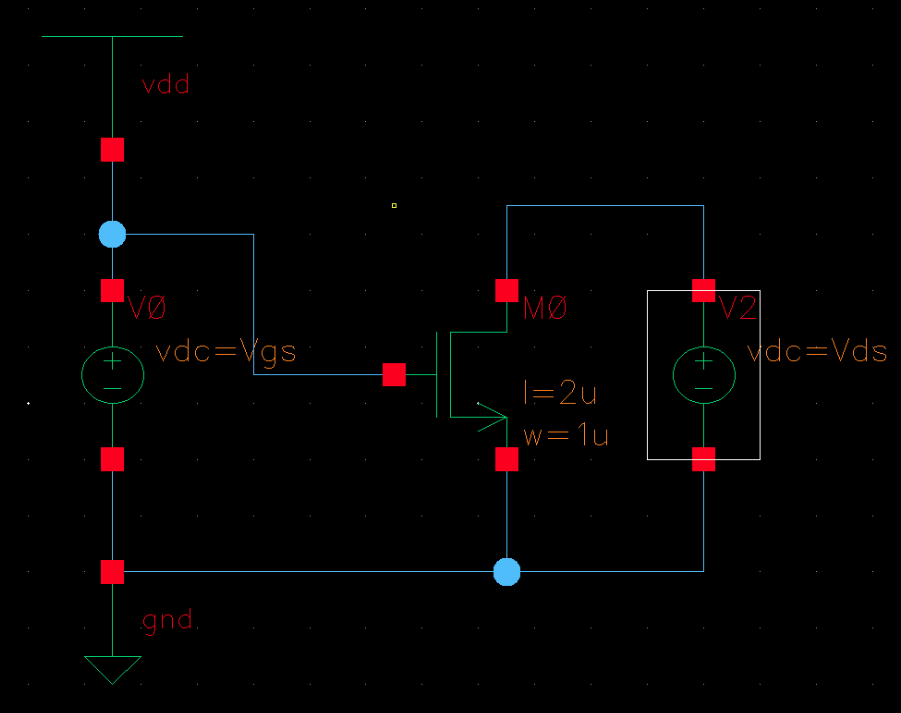
\includegraphics[width=0.8\textwidth]{task1/task1-schematic-nmos-sim.png}
  \caption{create new file}
\end{figure}

ADE L Setting

\begin{figure}[H]
  \centering
  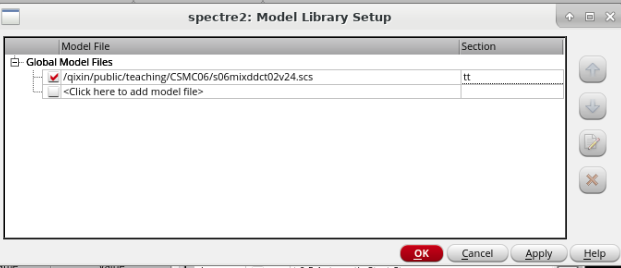
\includegraphics[width=0.8\textwidth]{task1/task1-ADE-L-model-library-setting.png}
  \caption{model-library-setting}
\end{figure}

\begin{figure}[H]
  \centering
  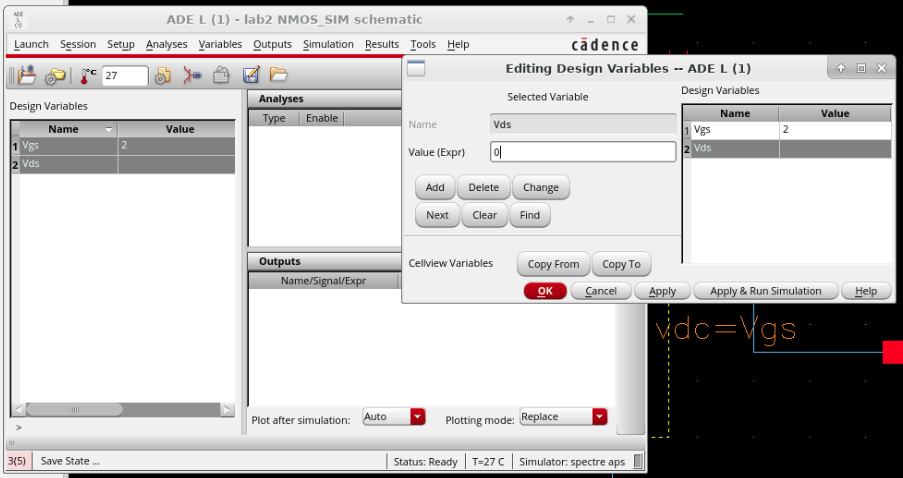
\includegraphics[width=0.8\textwidth]{task1/task1-ADE-L-setting-1.png}
  \caption{ADE L Setting 1}
\end{figure}

\begin{figure}[H]
  \centering
  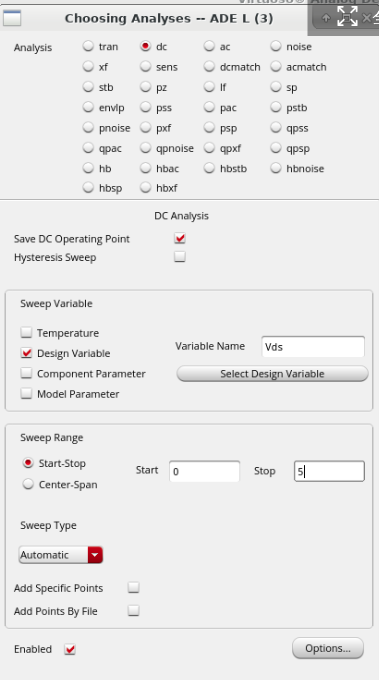
\includegraphics[width=0.8\textwidth]{task1/task1-ADE-L-setting-2.png}
  \caption{ADE L Setting 2}
\end{figure}

\begin{figure}[H]
  \centering
  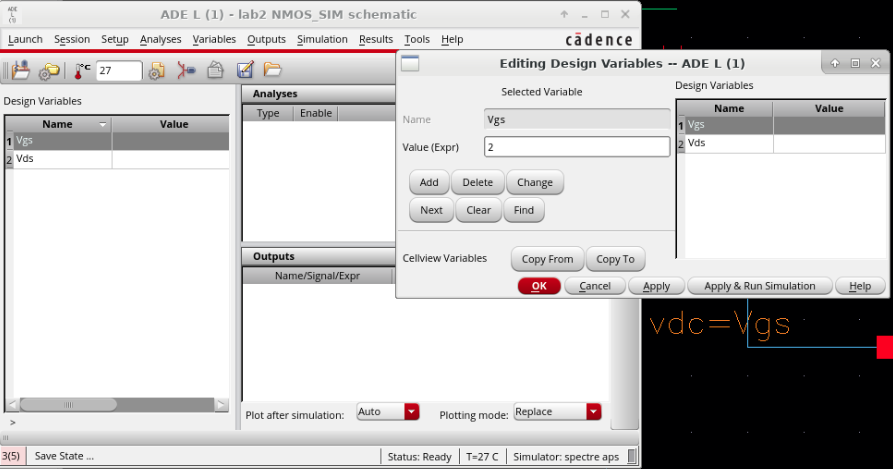
\includegraphics[width=0.8\textwidth]{task1/task1-ADE-L-setting-3.png}
  \caption{ADE L Setting 3}
\end{figure}

\begin{figure}[H]
  \centering
  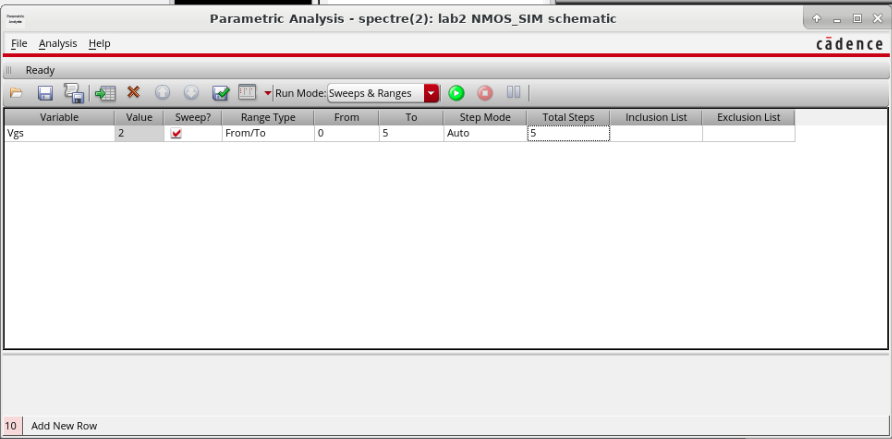
\includegraphics[width=0.8\textwidth]{task1/task1-ADE-L-setting-4.png}
  \caption{ADE L Setting 4}
\end{figure}

Save ADE L Setting

\begin{figure}[H]
  \centering
  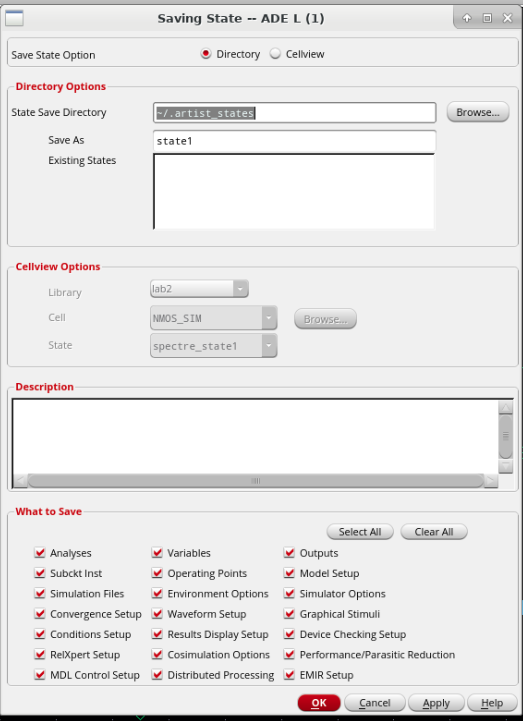
\includegraphics[width=0.8\textwidth]{task1/task1-ADE-L-model-library-setting-save.png}
  \caption{Save ADE L Setting}
\end{figure}

得到下列曲线

\begin{figure}[H]
  \centering
  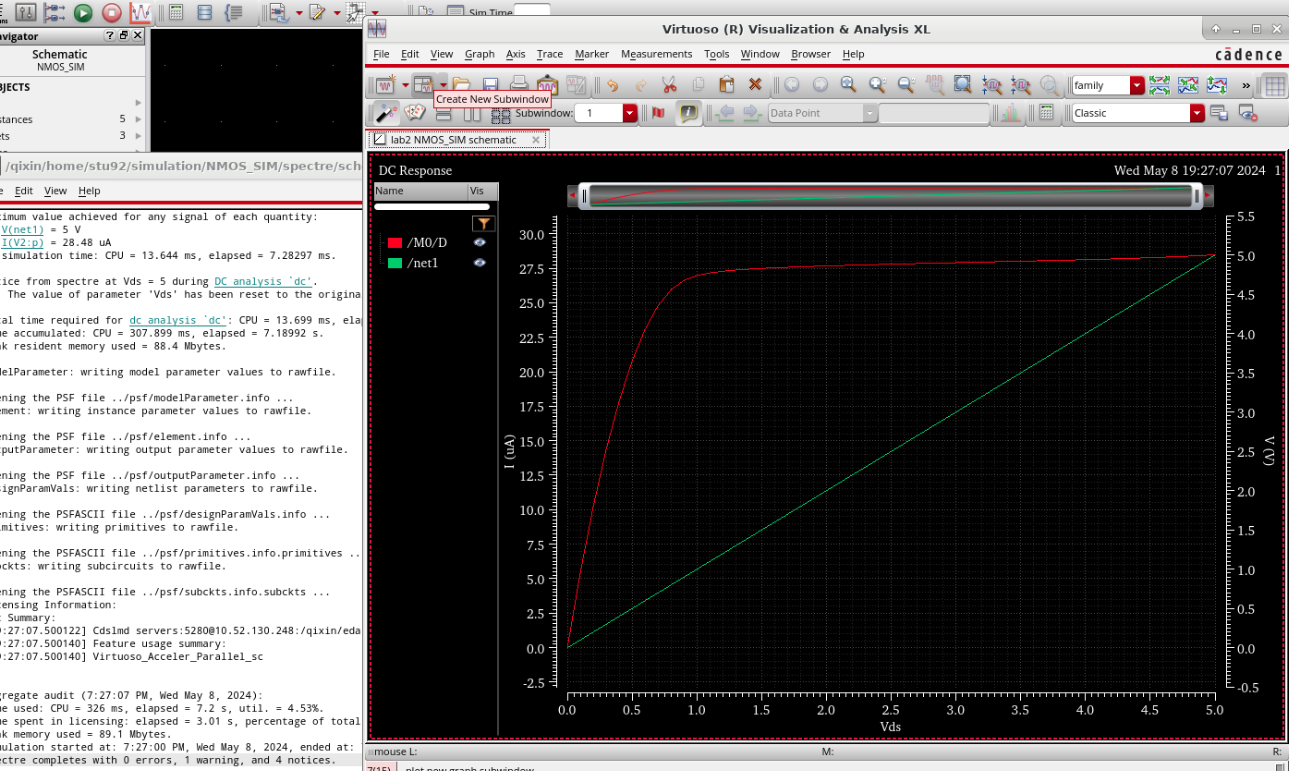
\includegraphics[width=0.8\textwidth]{task1/task1-plot-1.png}
  \caption{Plot 1}
\end{figure}

\begin{figure}[H]
  \centering
  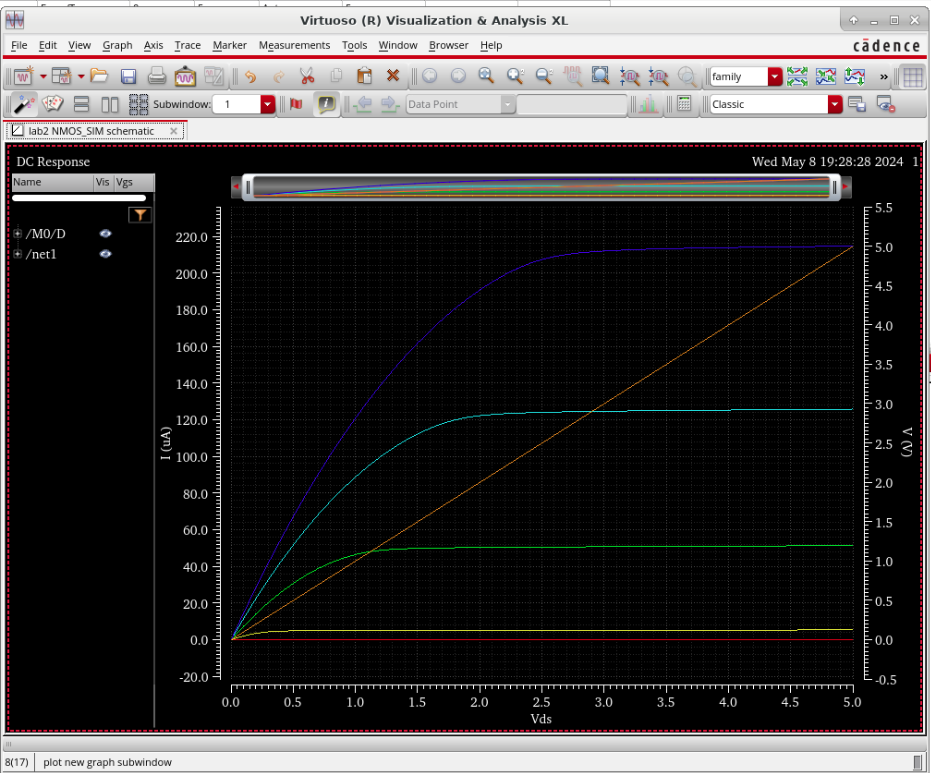
\includegraphics[width=0.8\textwidth]{task1/task1-plot-2.png}
  \caption{Plot 2}
\end{figure}

\subsection{任务2}

改变温度参数,从0变化到100度,得到不同曲线, 填写下表,并对比。

\begin{figure}[H]
  \centering
  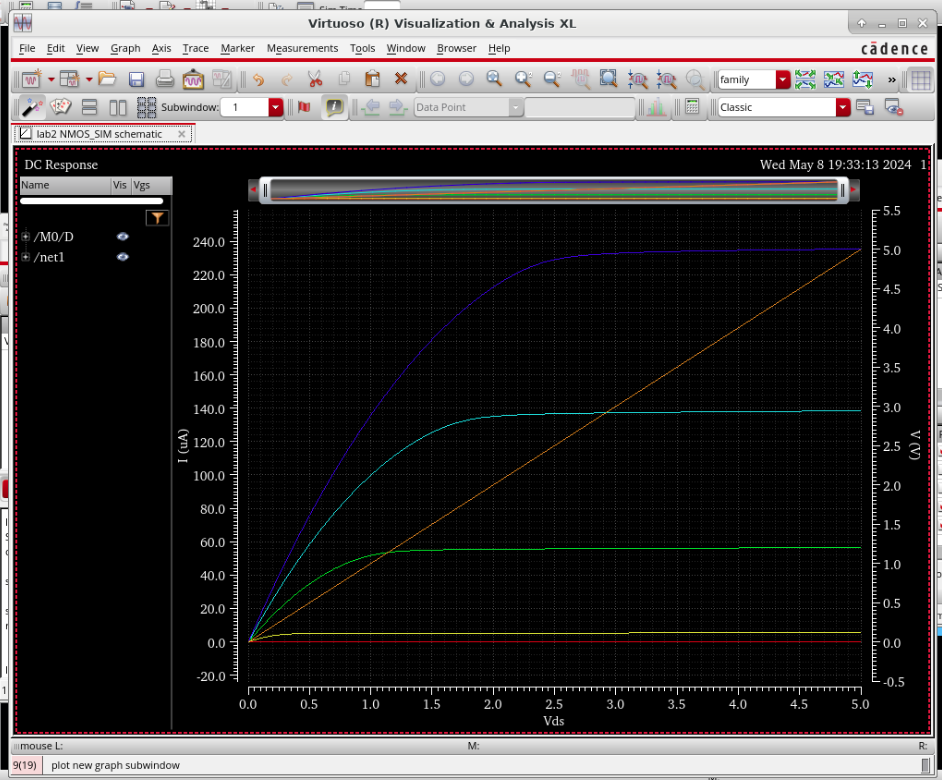
\includegraphics[width=0.6\textwidth]{task2/task2-t0-vgs18-vds4-2.png}
  \caption{T=0 Vgs=1.8V Vds=4V}
\end{figure}

\begin{figure}[htbp]
  \centering\begin{minipage}[t]{0.48\textwidth}
    \centering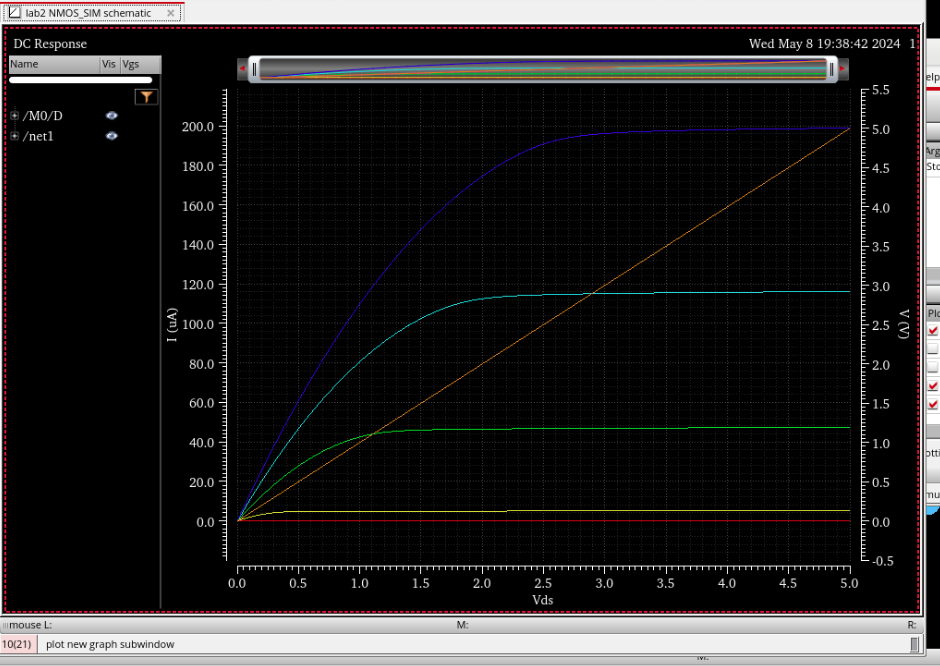
\includegraphics[width=0.9\textwidth]{task2/task2-t50-vgs18-vds4-2.png} 
    \caption{T=50 Vgs=1.8V Vds=4V}
  \end{minipage}
  \centering\begin{minipage}[t]{0.48\textwidth}
    \centering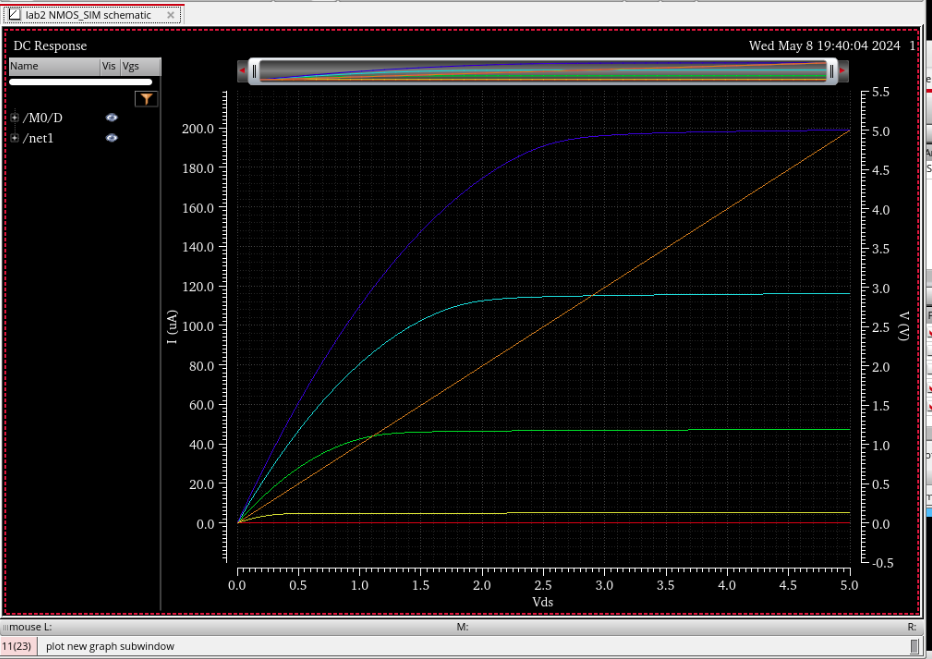
\includegraphics[width=0.9\textwidth]{task2/task2-t50-vgs18-vds8-2.png}
    \caption{T=50 Vgs=1.8V Vds=8V}
  \end{minipage}
  \\
  \centering\begin{minipage}[t]{0.48\textwidth}
    \centering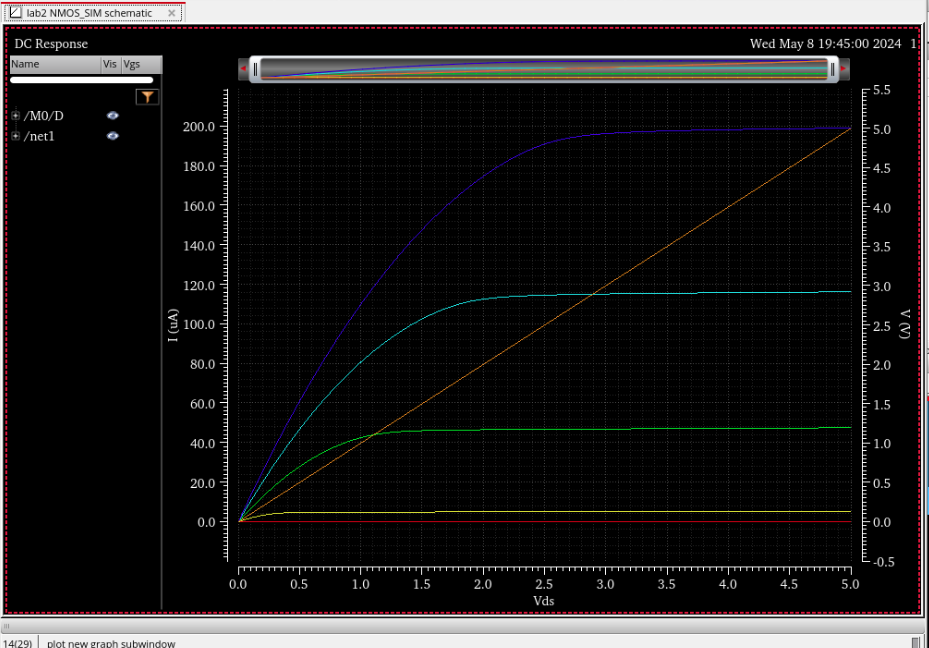
\includegraphics[width=0.9\textwidth]{task2/task2-t50-vgs22-vds4-2.png} 
    \caption{T=50, Vgs= 2.2V Vds=4V}
  \end{minipage}
  \centering\begin{minipage}[t]{0.48\textwidth}
    \centering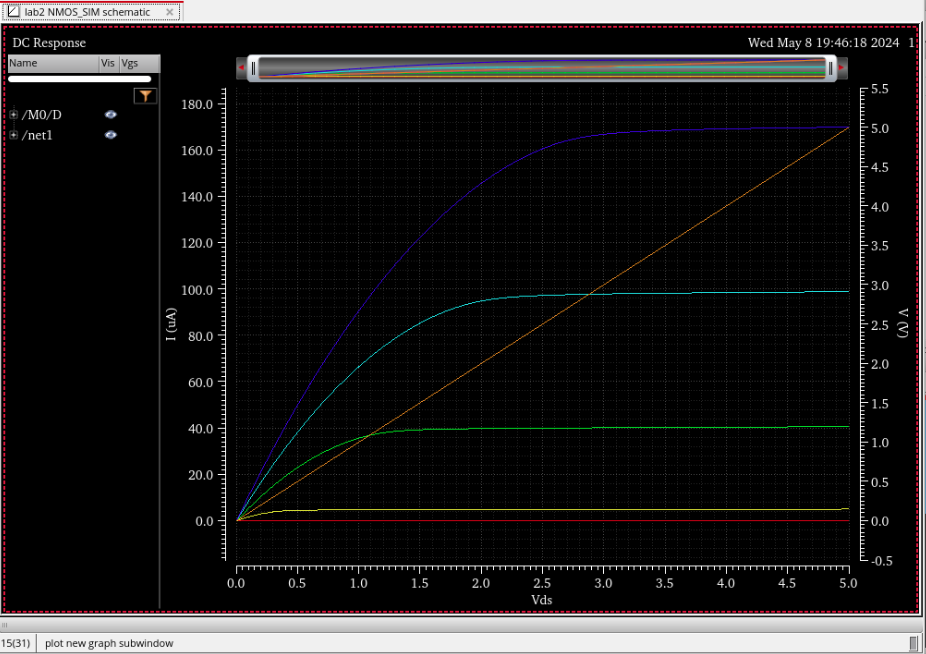
\includegraphics[width=0.9\textwidth]{task2/task2-t100-vgs22-vds4-2.png}
    \caption{T=100 Vgs=2.2V Vds=4V}
  \end{minipage}
\end{figure}

\subsection{任务3}

CMOS反相器的直流(DC)仿真  nmos4, pmos4

ADE窗口中加模型库

\begin{figure}[H]
  \centering
  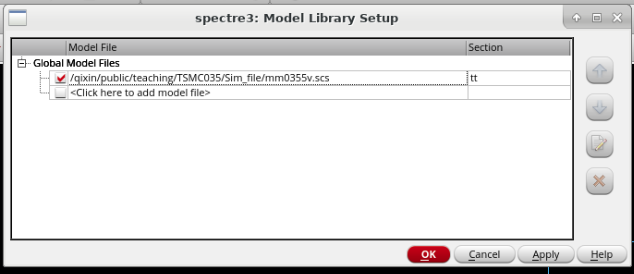
\includegraphics[width=0.8\textwidth]{task3/task3-ADE-L-model-library-setup.png}
  \caption{ADE窗口中加模型库}
\end{figure}

绘制原理图

\begin{figure}[H]
  \centering
  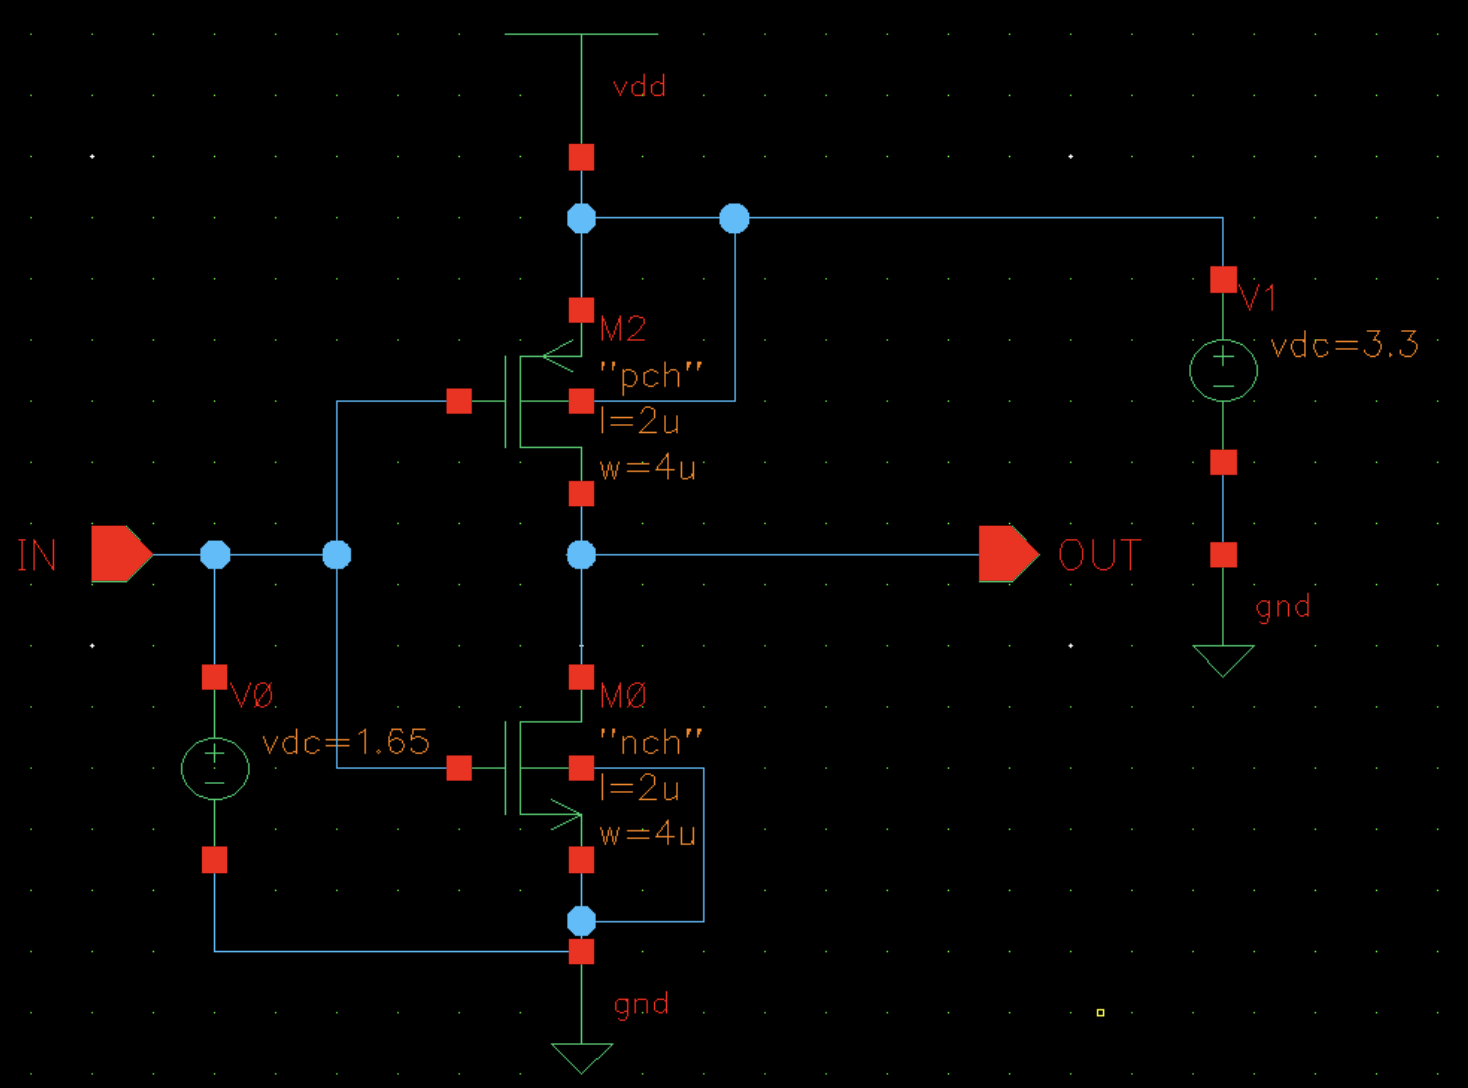
\includegraphics[width=0.8\textwidth]{task3/task3-inverter-sim-layout.png}
  \caption{原理图}
\end{figure}

进行直流分析

Select Component 原理图中选择V0

\begin{figure}[htbp]
  \centering\begin{minipage}[t]{0.48\textwidth}
    \centering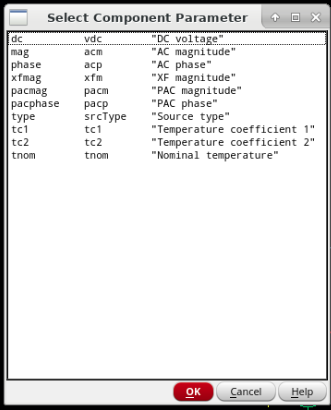
\includegraphics[width=0.9\textwidth]{task3/task3-Select-Component-Parameter.png}
    \caption{设置}
  \end{minipage}
  \centering\begin{minipage}[t]{0.48\textwidth}
    \centering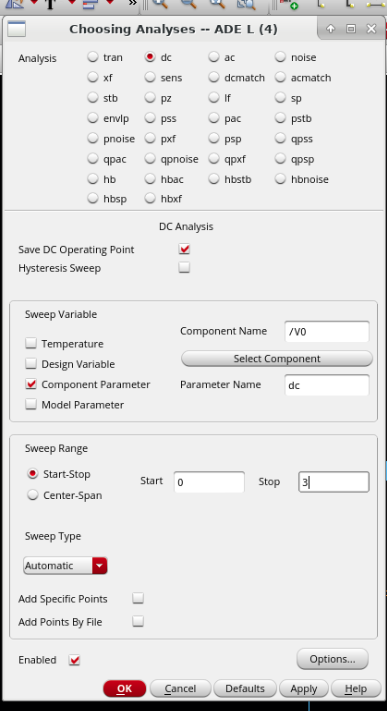
\includegraphics[width=0.9\textwidth]{task3/task3-choosing-analyse.png}
    \caption{设置}
  \end{minipage}
\end{figure}

\begin{figure}[H]
  \centering
  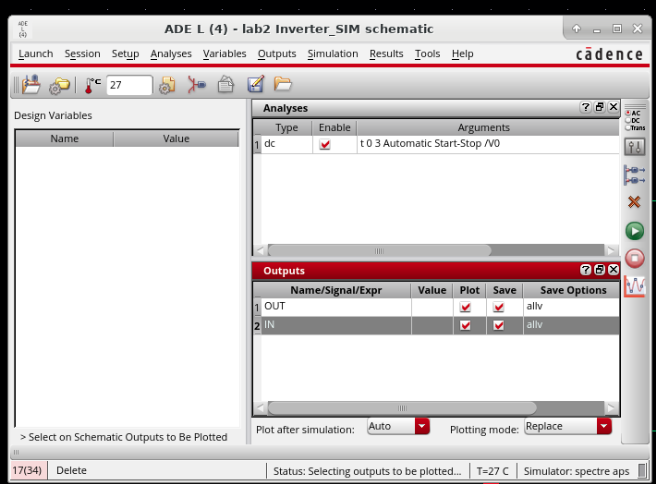
\includegraphics[width=0.8\textwidth]{task3/task3-ADE-L-settings.png}
  \caption{设置}
\end{figure}

得到下列曲线

\begin{figure}[H]
  \centering
  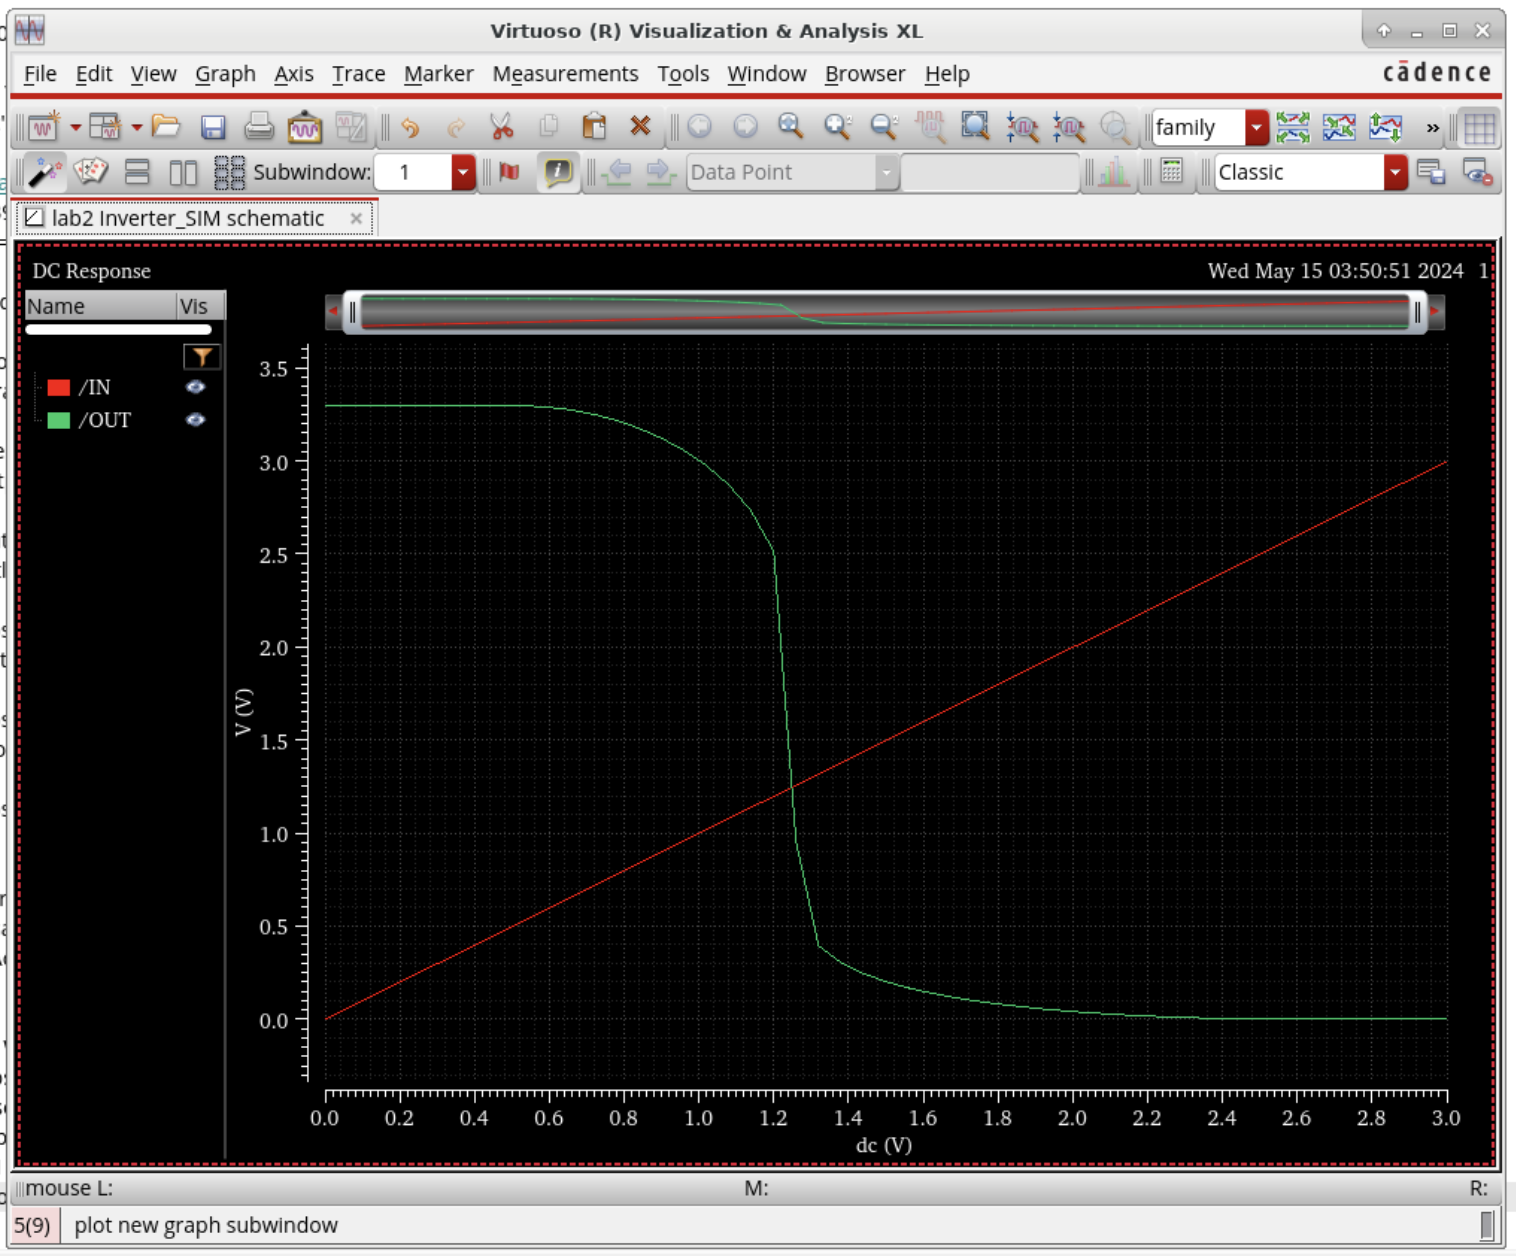
\includegraphics[width=0.8\textwidth]{task3/task3-analyse-plot.png}
  \caption{Plot}
\end{figure}

\subsection{任务4}

1 准备工作

复制 \texttt{/qixin/project/library/smic180nm\_ms/smic18mse\_1833\_\dots} 中的 \texttt{display.drf} 到 
\texttt{/qixin/home/stuXX/Desktop/202xXXXX/lab2/123/} 中。

修改(如果没有的话就新建一个) \texttt{cds.lib} 文件,添加模型库路径

\texttt{DEFINE smic18mmrf /qixin/project/library/smic180nm\_ms/smic180mse\_1833\_1P6M\_5Ia\_1TMa1\_MIM10\_oa\_cds\_2019\_01\_15\_v1.11\_4/smic18mmrf}

\begin{figure}[H]
  \centering
  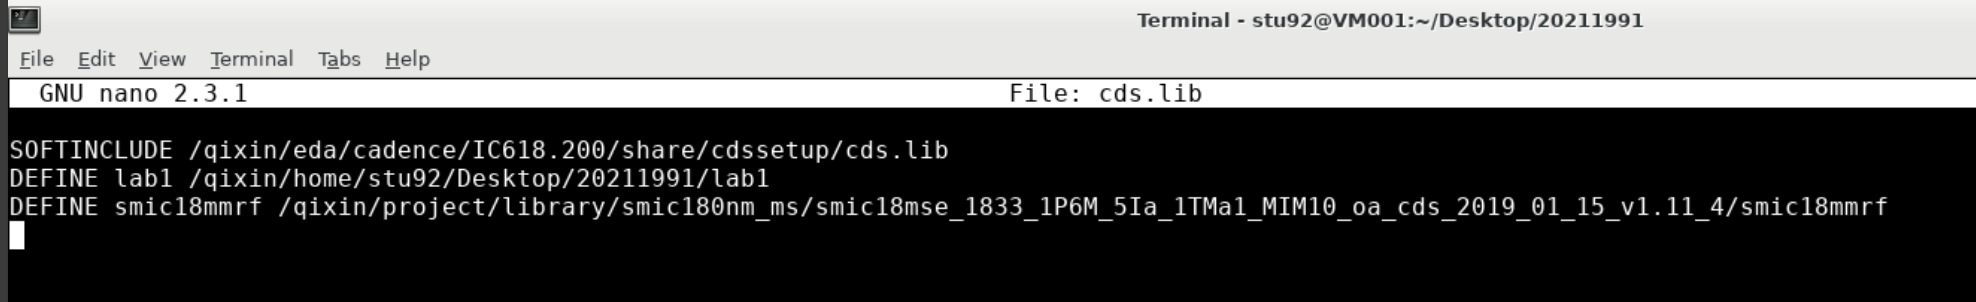
\includegraphics[width=0.8\textwidth]{task4/task4-preparation-1.png}
  \caption{Edit cds.lib}
\end{figure}

启动环境 \texttt{virtuoso \&}

在 library manager 窗口中,确认 smic18mmrf 在 library 这一栏里面。勾选 \texttt{Show Categories}。

\begin{figure}[H]
  \centering
  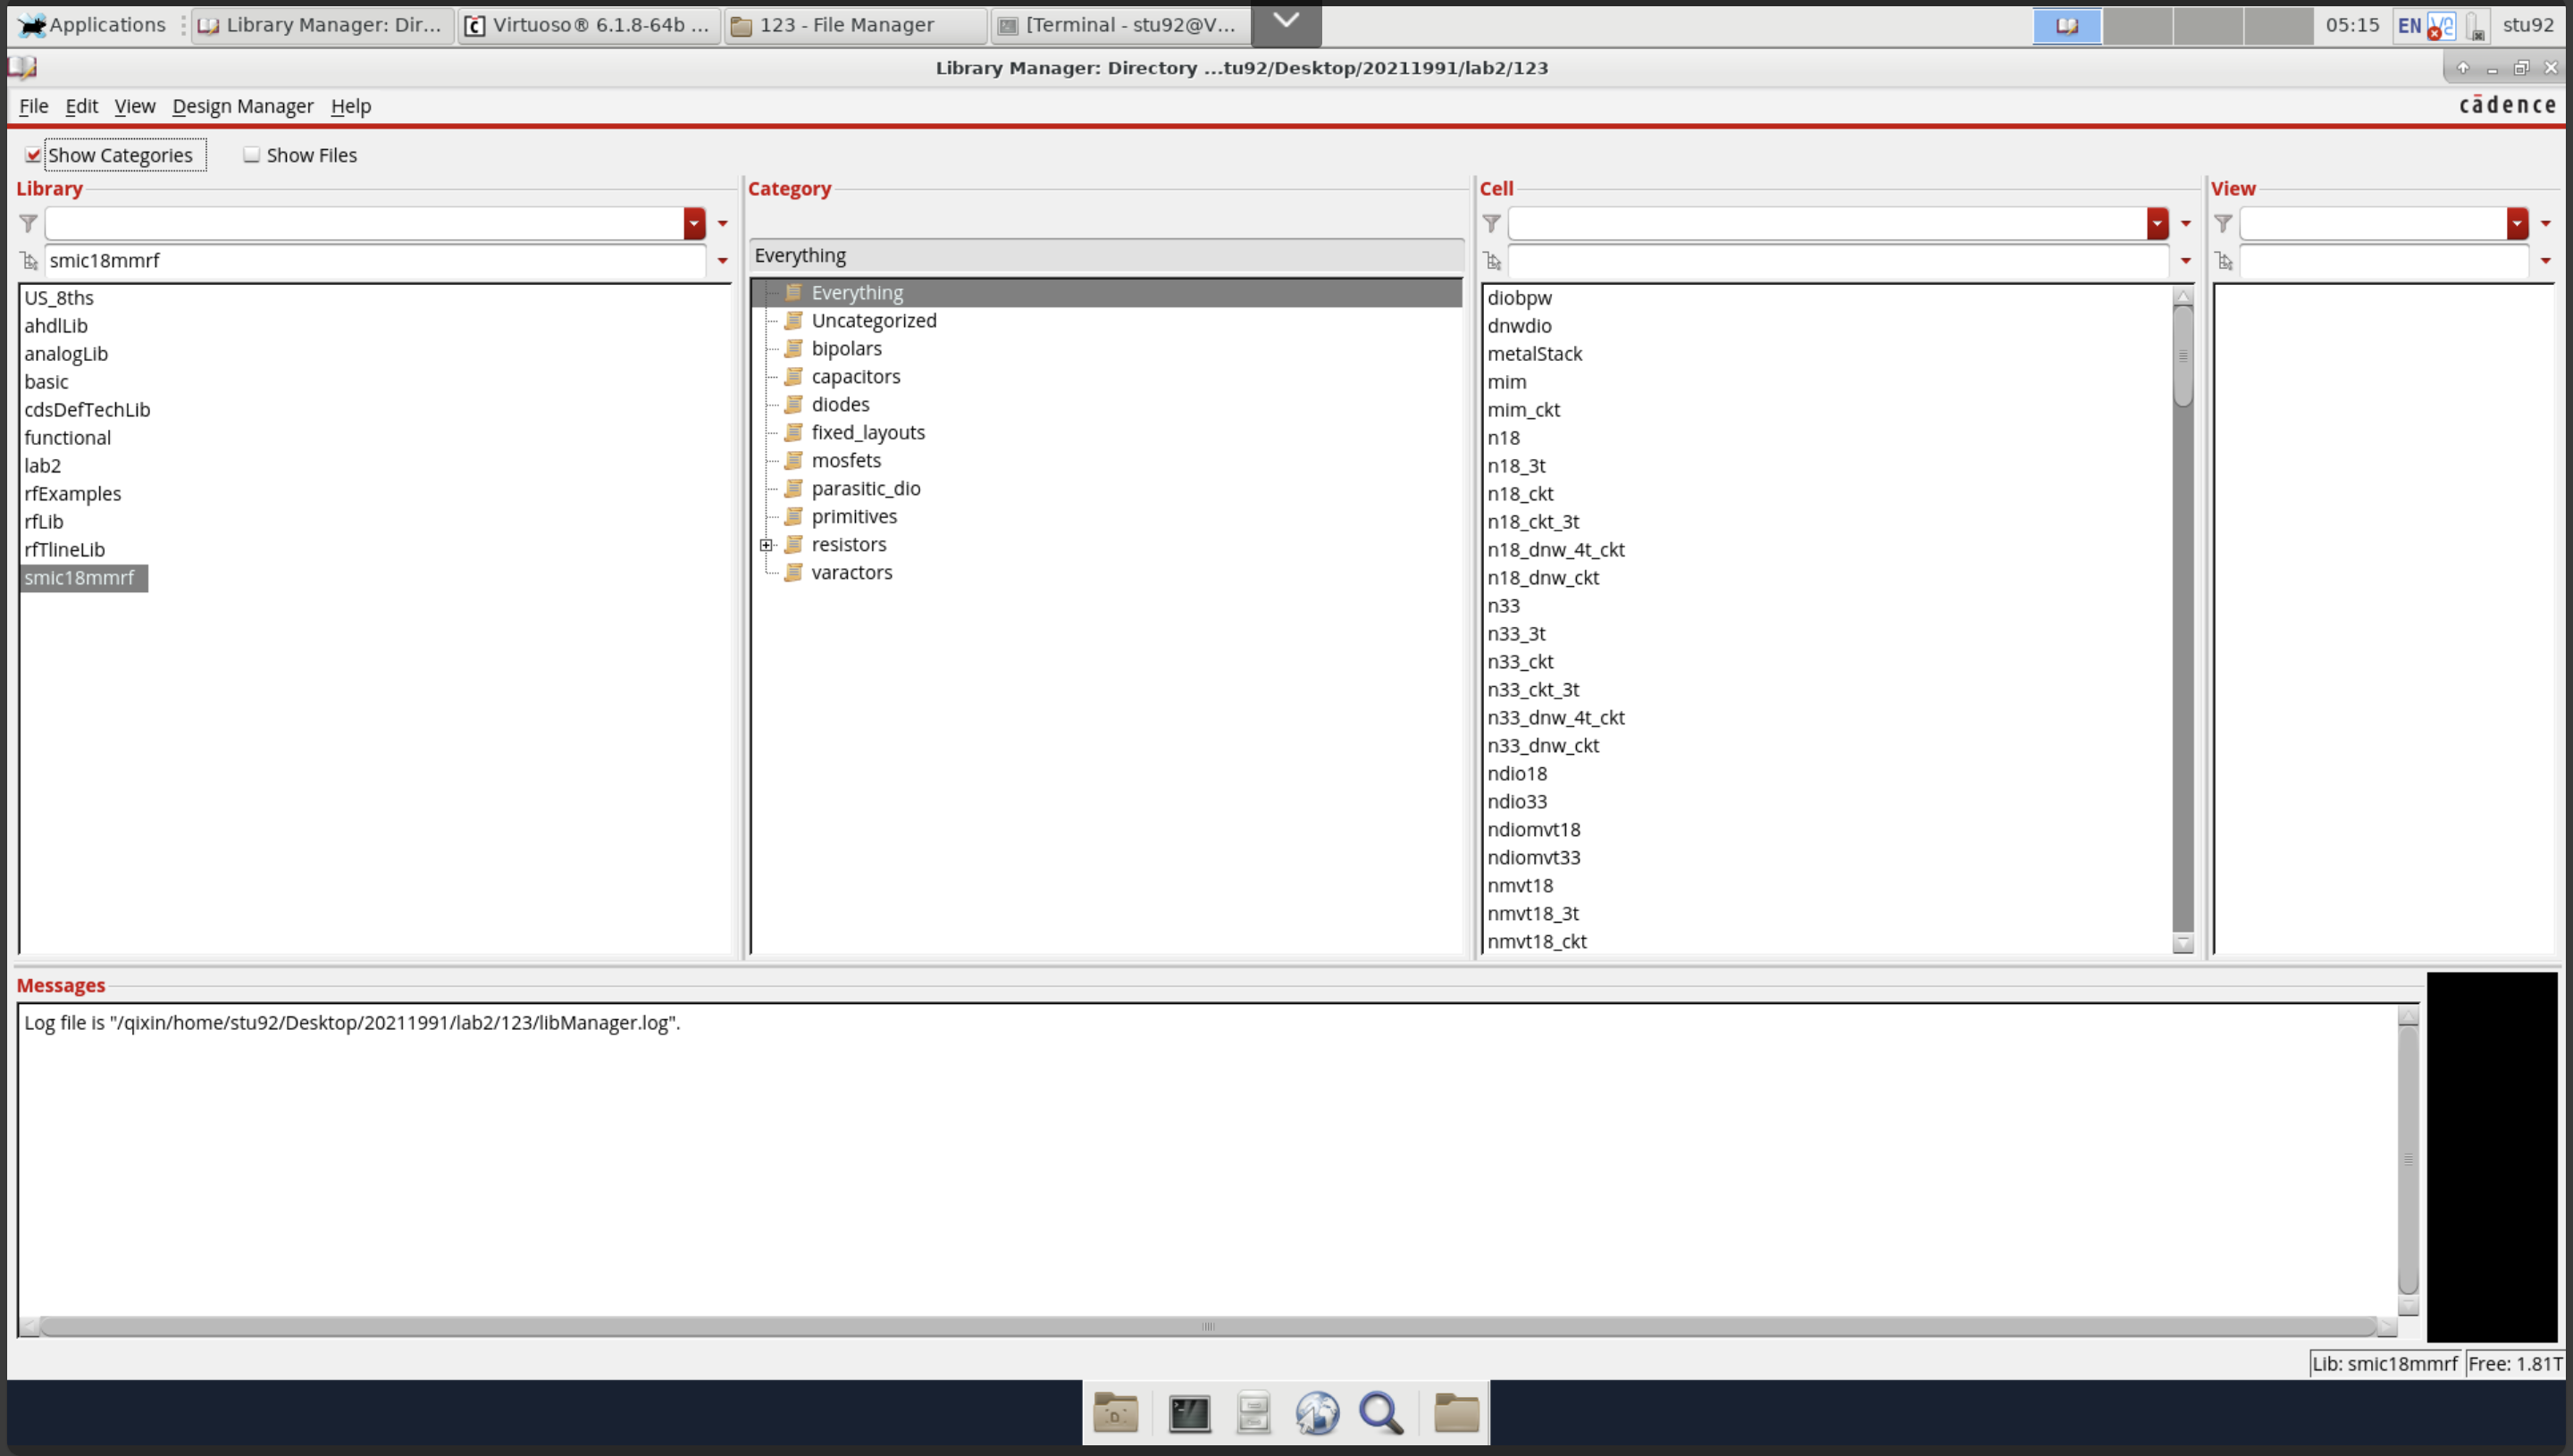
\includegraphics[width=0.8\textwidth]{task4/task4-preparation-2.png}
  \caption{Check Library Manager}
\end{figure}

2 连接CMOS反相器的原理图,并生成它的符号图

\begin{figure}[htbp]
  \centering\begin{minipage}[t]{0.48\textwidth}
    \centering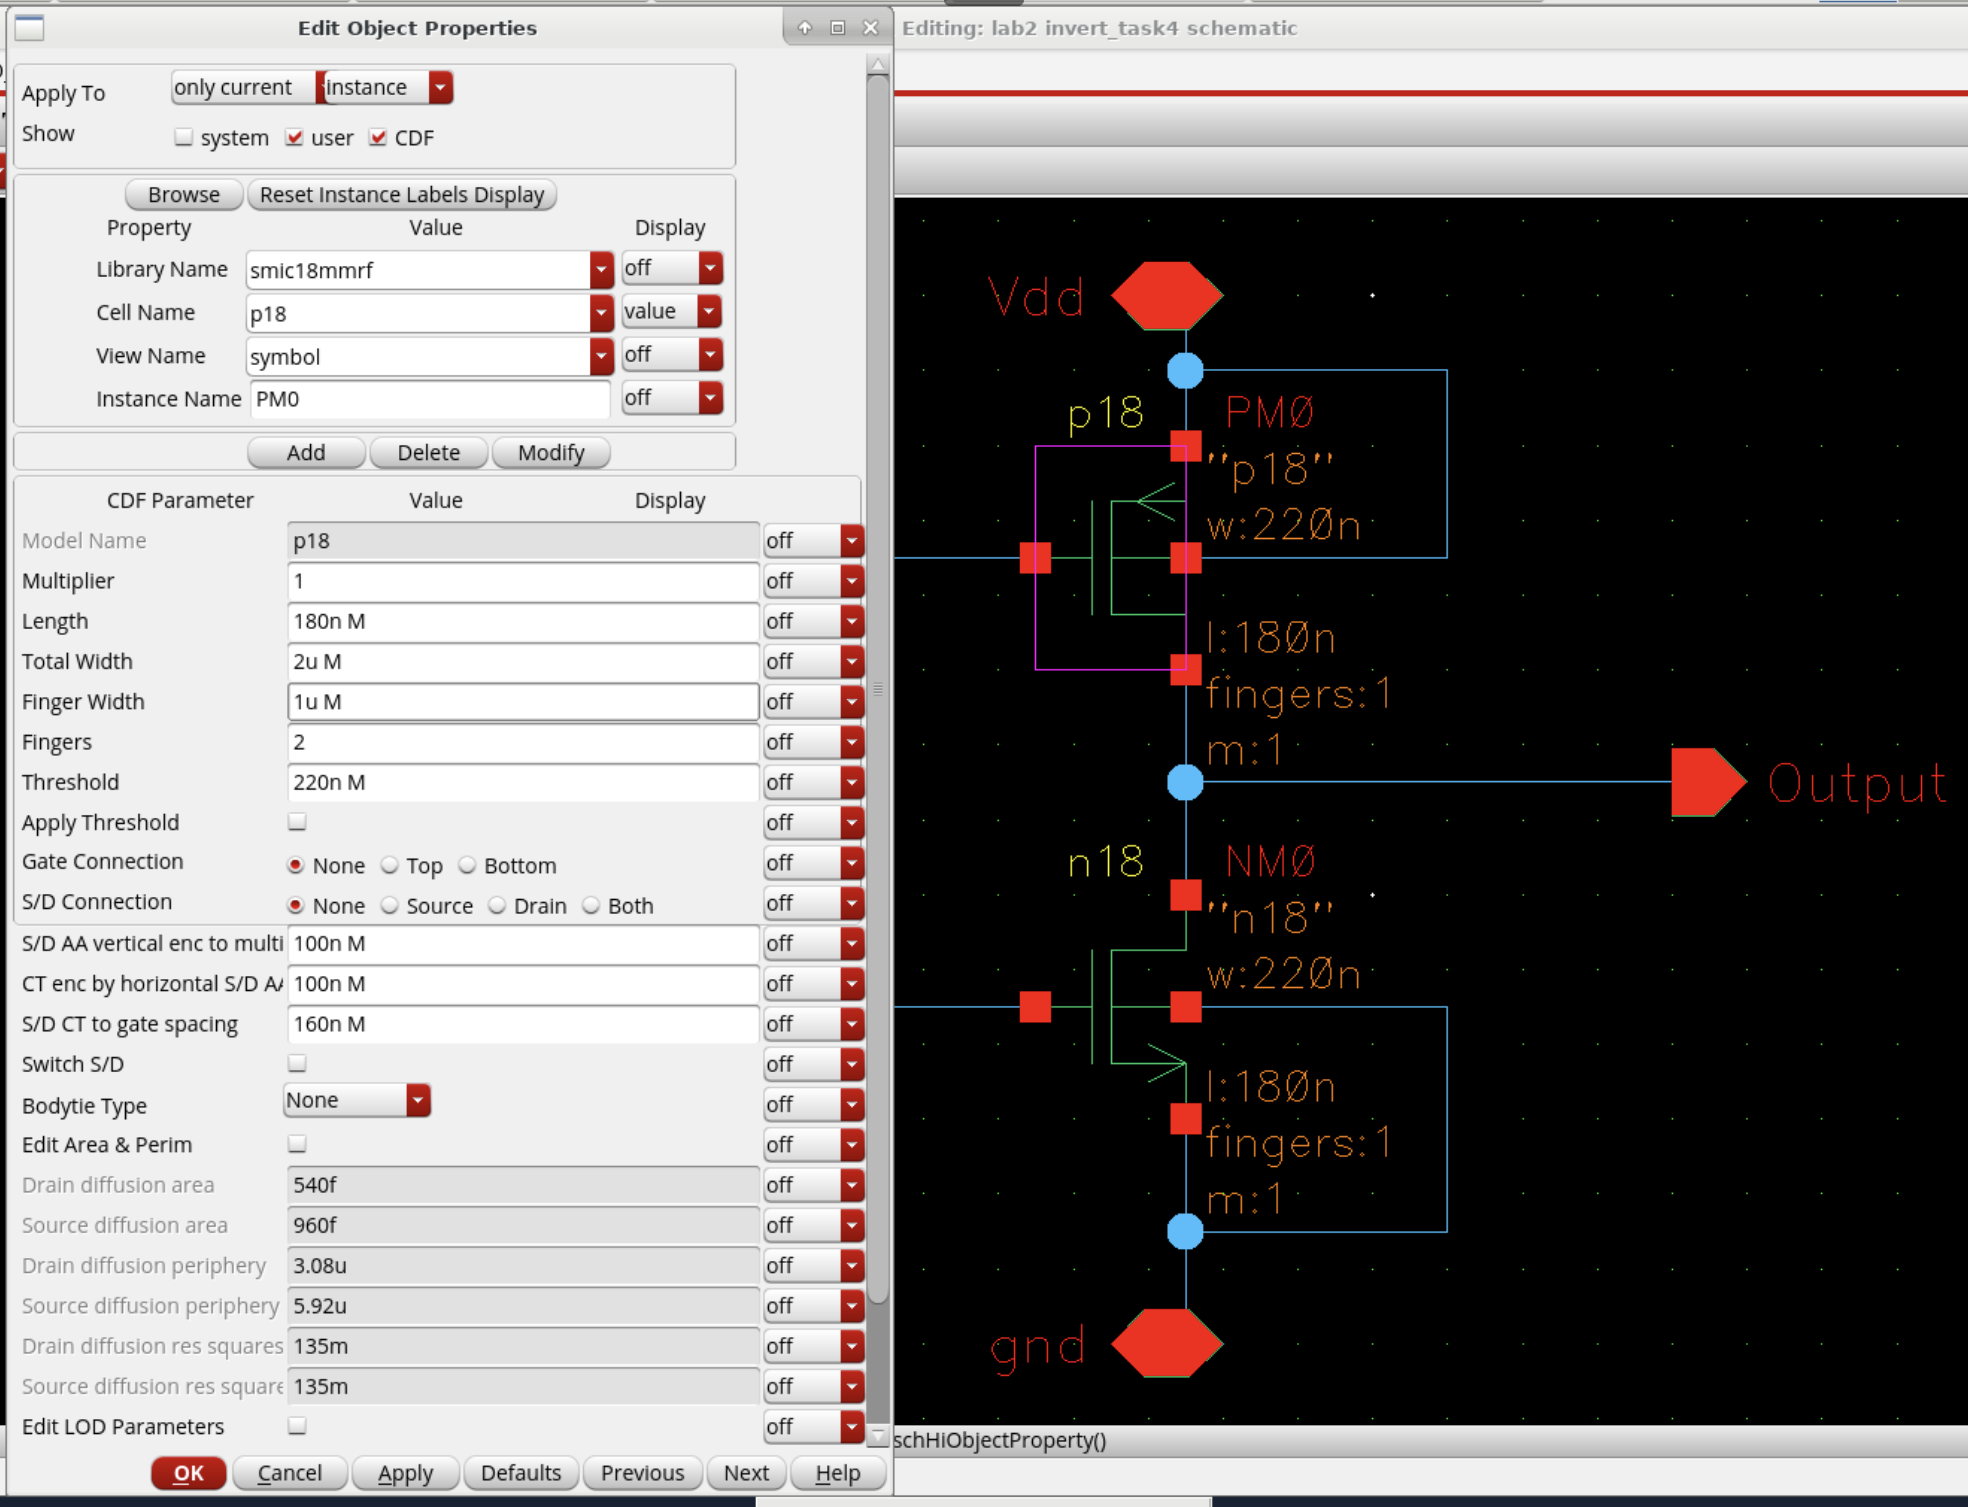
\includegraphics[width=0.9\textwidth]{task4/task4-layout-invert-para-1.png}
    \caption{Edit p18}
  \end{minipage}
  \centering\begin{minipage}[t]{0.48\textwidth}
    \centering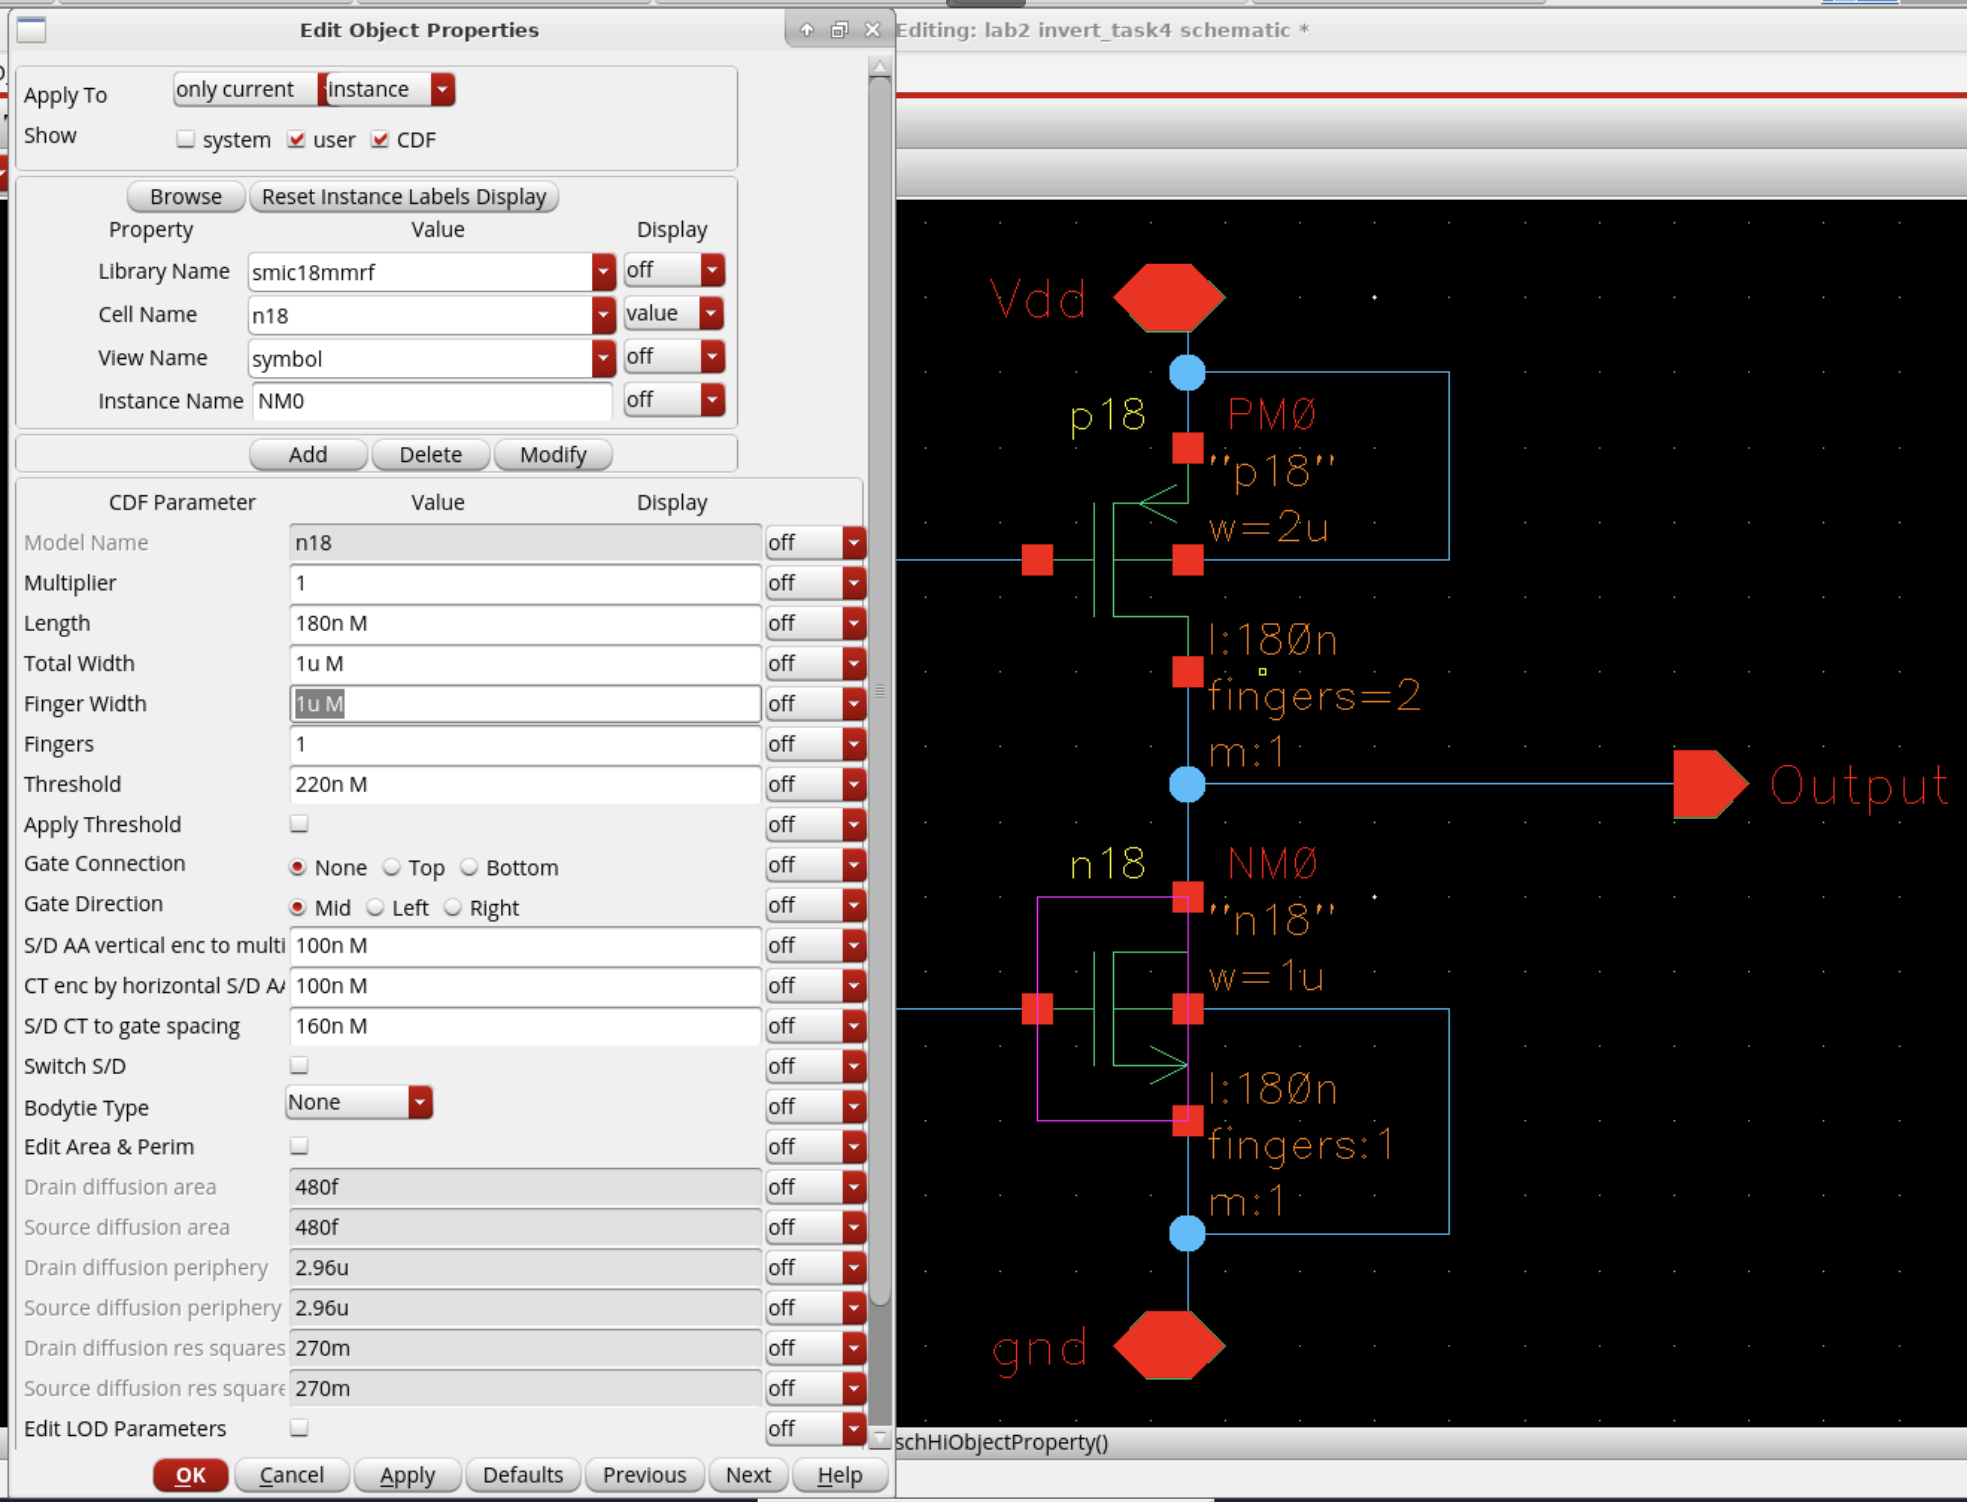
\includegraphics[width=0.9\textwidth]{task4/task4-layout-invert-para-2.png}
    \caption{Edit n18}
  \end{minipage}
\end{figure}

最后完成的 layout

\begin{figure}[H]
  \centering
  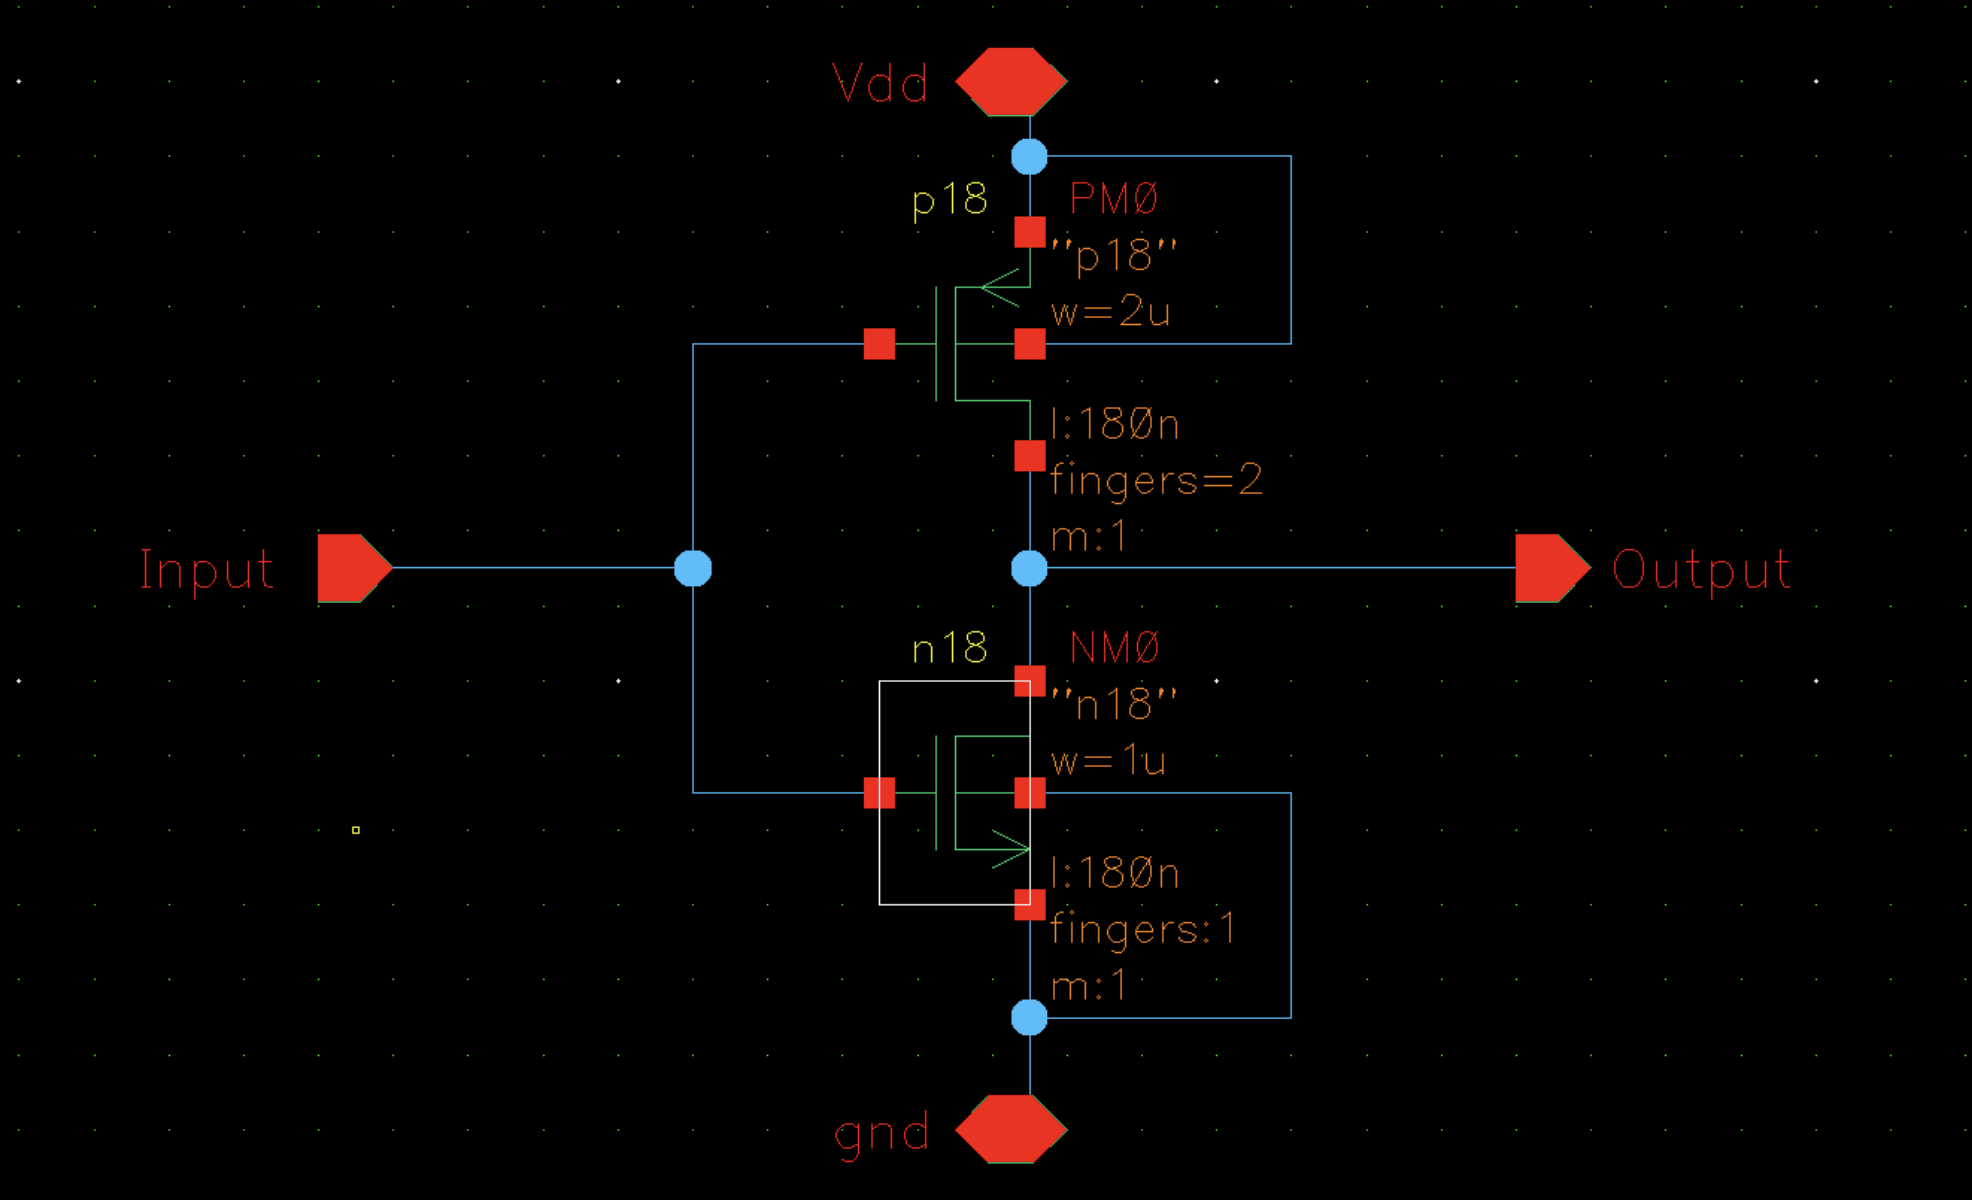
\includegraphics[width=0.8\textwidth]{task4/task4-layout-invert.png}
  \caption{Task4 invert layout}
\end{figure}

3 调用反相器的符号图,建立测试原理图。

\begin{figure}[H]
  \centering
  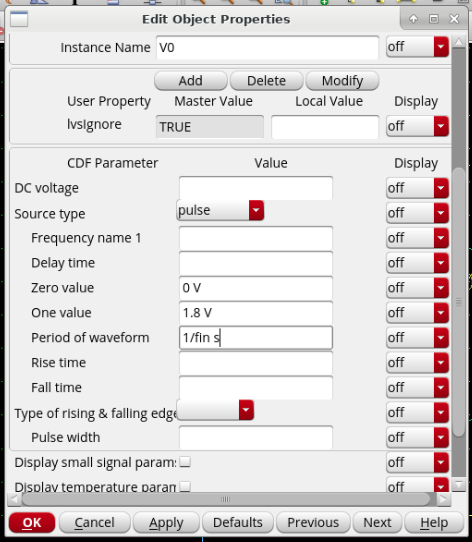
\includegraphics[width=0.8\textwidth]{task4/task4-layout-inverter-tb-para-1.png}
  \caption{Task4 invert layout}
\end{figure}

\begin{figure}[H]
  \centering
  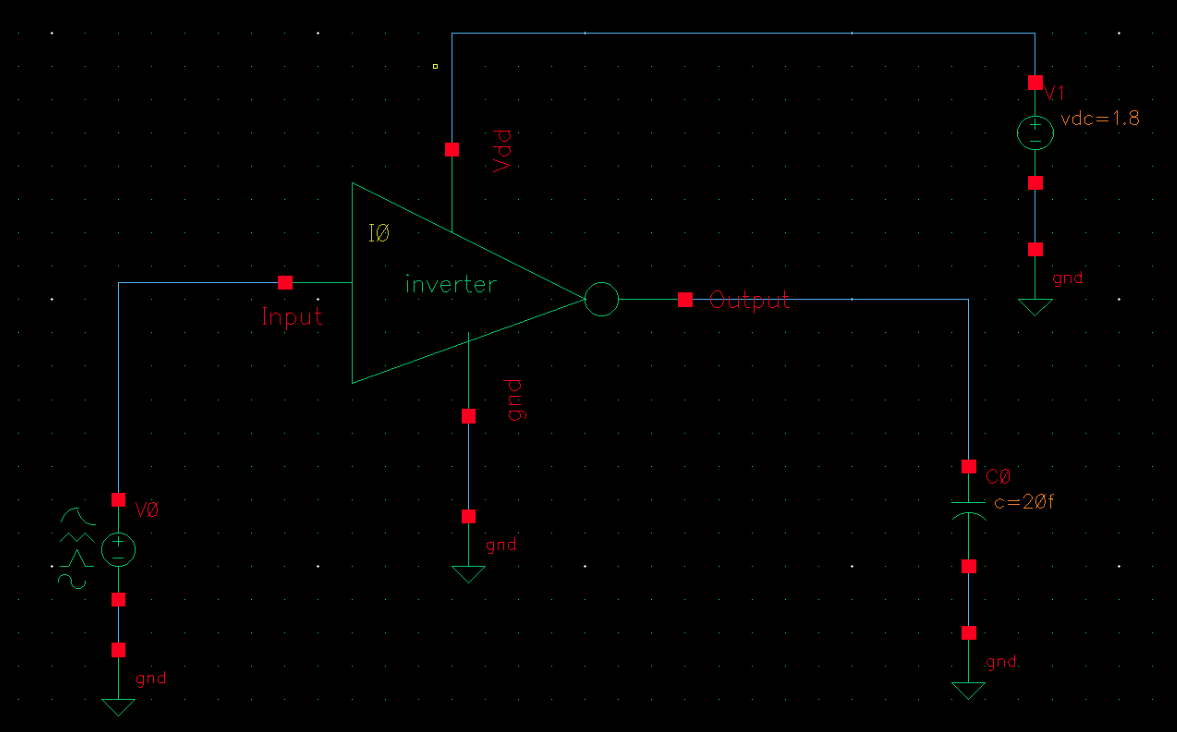
\includegraphics[width=0.8\textwidth]{task4/task4-layout-inverter-tb.png}
  \caption{Task4 invert layout}
\end{figure}

仿真环境设置:

模型路径

\begin{figure}[htbp]
  \centering\begin{minipage}[t]{0.48\textwidth}
    \centering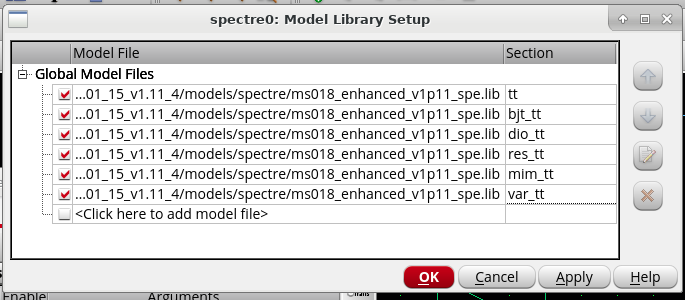
\includegraphics[width=0.9\textwidth]{task4/task4-inverter-tb-ADE-L-setting-1.png}
    \caption{Task4 Mobel Library Setting}
  \end{minipage}
  \centering\begin{minipage}[t]{0.48\textwidth}
    \centering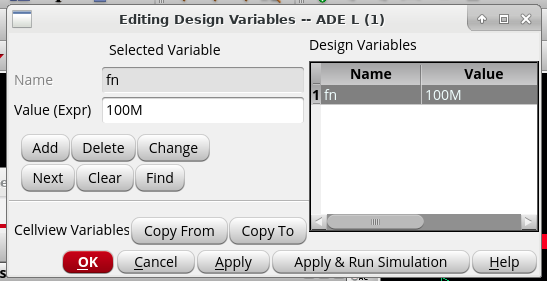
\includegraphics[width=0.9\textwidth]{task4/task4-inverter-tb-ADE-L-setting-2.png}
    \caption{Task4 Mobel Library Setting - fn}
  \end{minipage}
  \\
  \centering\begin{minipage}[t]{0.48\textwidth}
    \centering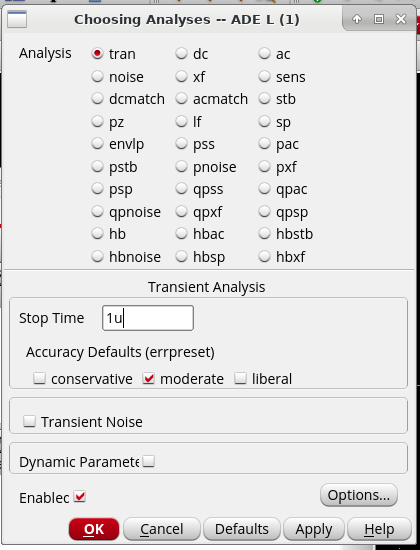
\includegraphics[width=0.9\textwidth]{task4/task4-inverter-tb-ADE-L-setting-3.png}
    \caption{Task4 Choosing Analyse}
  \end{minipage}
  \centering\begin{minipage}[t]{0.48\textwidth}
    \centering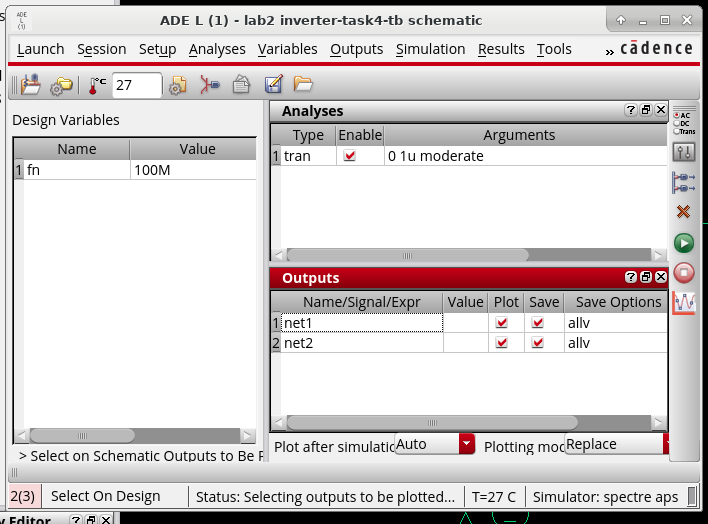
\includegraphics[width=0.9\textwidth]{task4/task4-inverter-tb-ADE-L-setting-4.png}
    \caption{Task4 ADE L Setting}
  \end{minipage}
\end{figure}

Run and have the wave view

\begin{figure}[H]
  \centering
  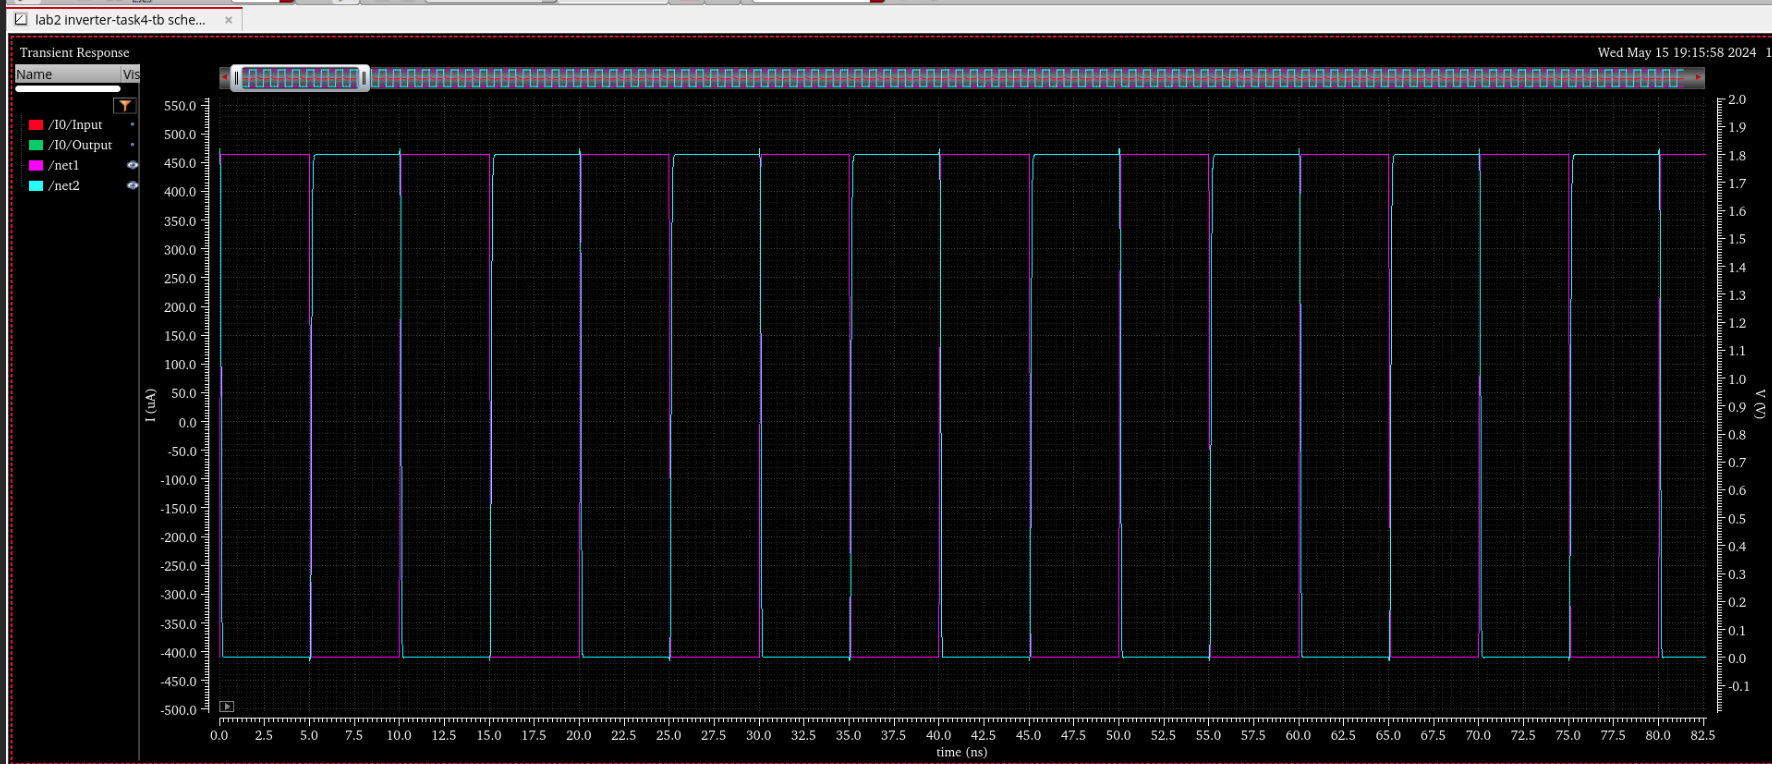
\includegraphics[width=0.8\textwidth]{task4/task4-inverter-tb-wave-1.png}
  \caption{Wava 1}
\end{figure}

split图形,分开显示

\begin{figure}[H]
  \centering
  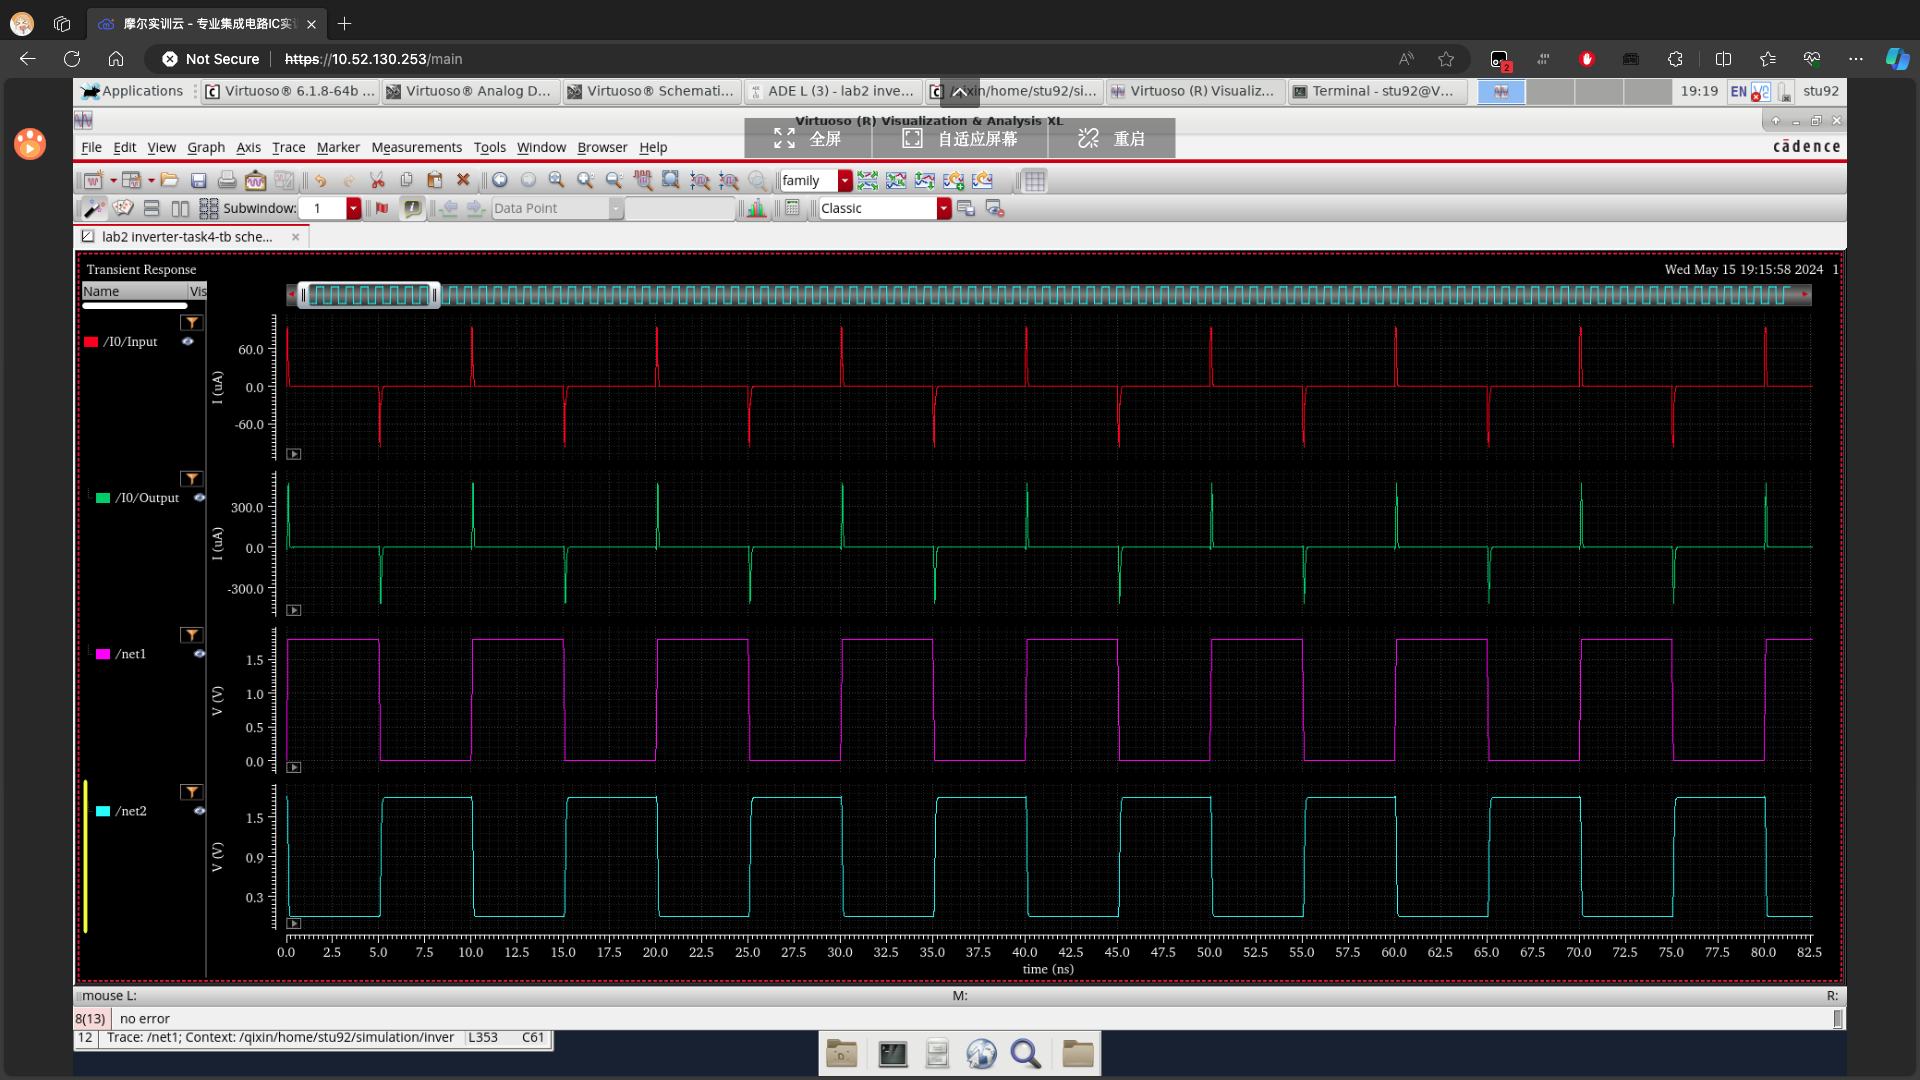
\includegraphics[width=0.8\textwidth]{task4/task4-inverter-tb-wave-2.png}
  \caption{Wava 1 Split}
\end{figure}

合并到一个框,继续拉大,可见输入输出电压上升和下降的细节

\begin{figure}[H]
  \centering
  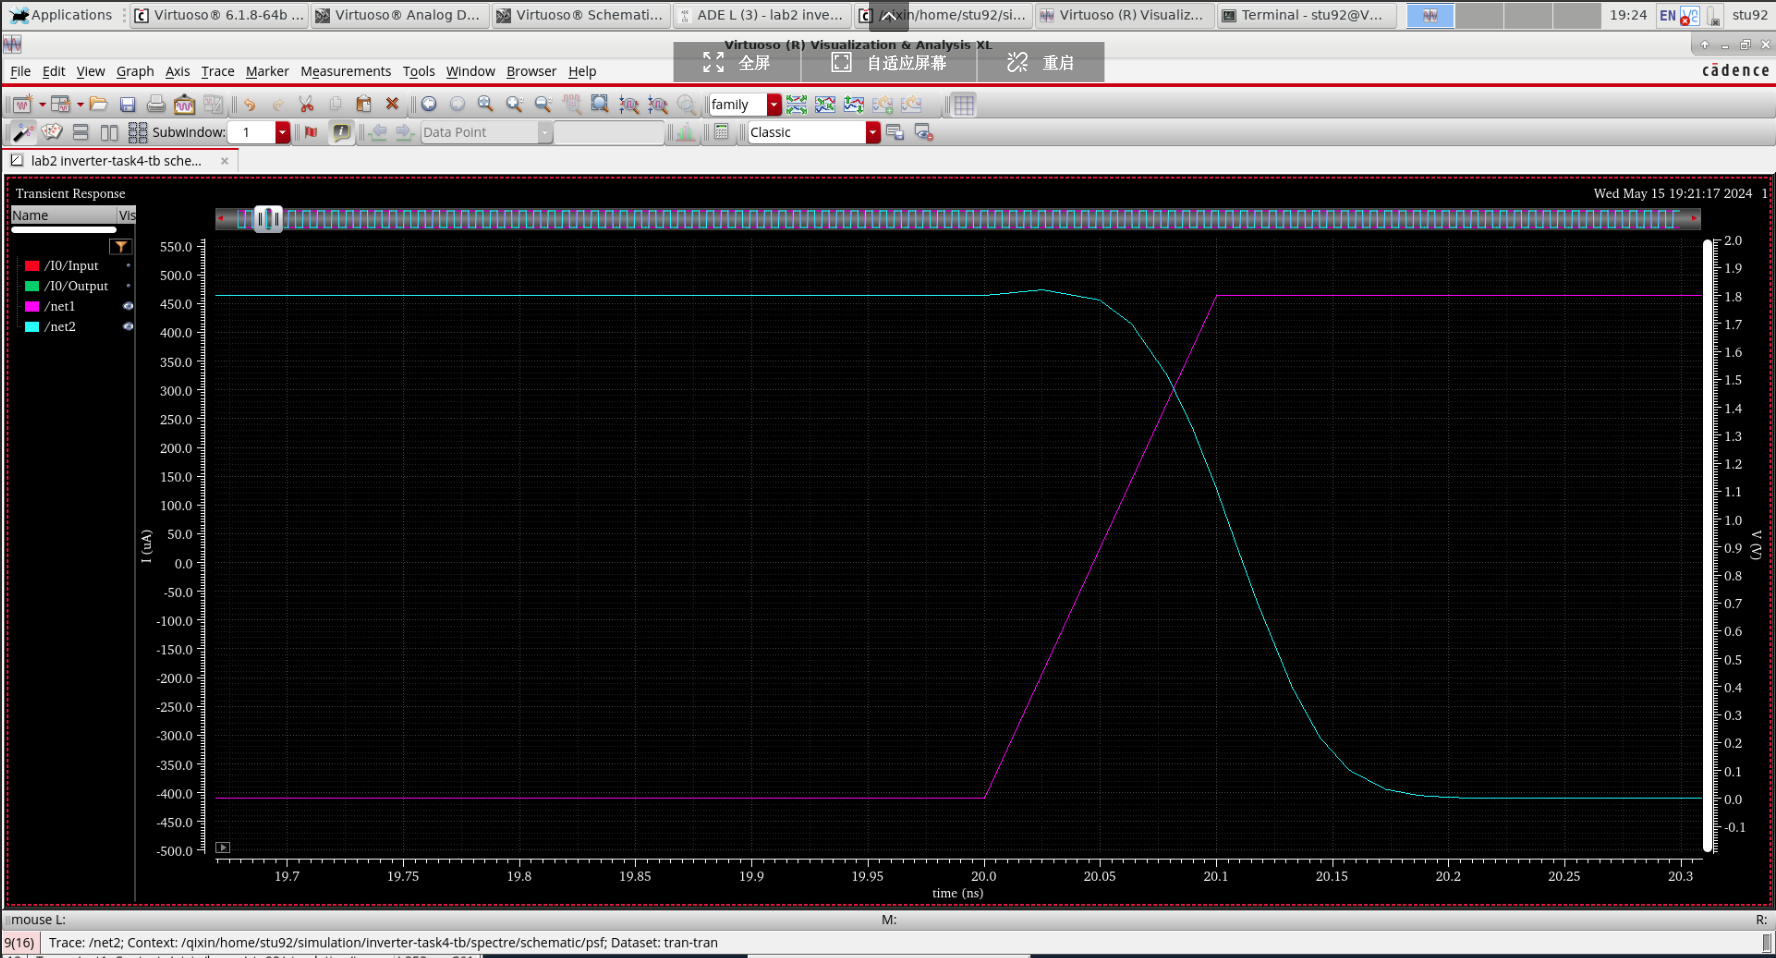
\includegraphics[width=0.8\textwidth]{task4/task4-inverter-tb-wave-3.png}
  \caption{Wava 1 Zoom}
\end{figure}

按 \texttt{a} 键在输入曲线上打标签,按 \texttt{b} 键在输出曲线上打标签,请回答

问题1:这两点构成的水平线段代表什么含义?

\begin{figure}[H]
  \centering
  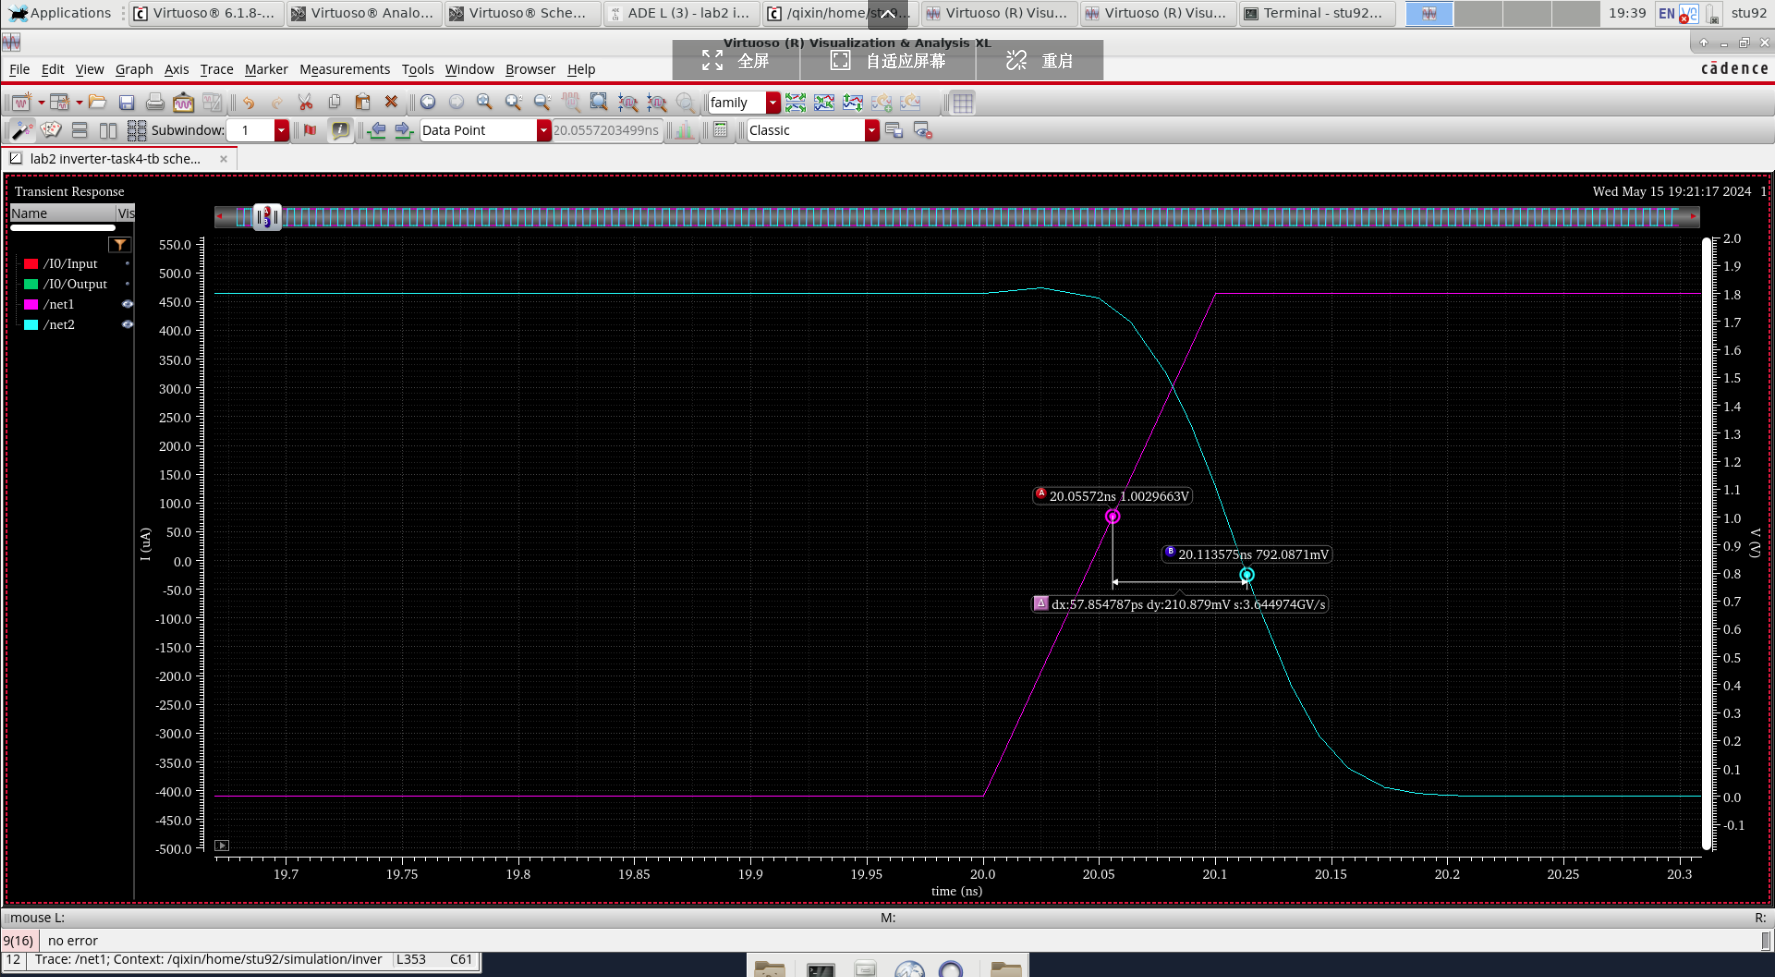
\includegraphics[width=0.8\textwidth]{task4/task4-inverter-tb-wave-4.png}
  \caption{Question 1}
\end{figure}

反相器输入输出曲线,观察波形图,在输入上升与输出下降区域,分别标记A点和B点,计算得到A点和B点的坐标如下:

A点:20.05572ns 1002.9663mV(在输入信号)
B点:20.113575ns 792.0871mV(在输出信号)

1. $A_x - B_x$:代表输入信号变化到特定电压值(A点)与输出信号响应到相应电压值(B点)之间的时间差。这可以用来表示反相器的传播延迟(propagation delay)。计算如下:

   \[
   A_x - B_x = 20.05572\text{ns} - 20.113575\text{ns} = -57.855\text{ps}
   \]

   这个负值表明,输入信号达到A点所需的时间比输出信号达到B点所需的时间要早,说明反相器在输入信号变化后有一定的延迟才会在输出信号上反映出来。

2. $A_y - B_y$:代表输入信号和输出信号之间的电压差。这个值可以用于评估反相器的电压摆幅(voltage swing)或电压响应。计算如下:

   \[
   A_y - B_y = 1002.9663\text{mV} - 792.0871\text{mV} = 210.8792\text{mV}
   \]

   这个电压差表示输入信号从792.0871mV增加到1002.9663mV的过程中,输出信号在相应时间段内的电压变化。

总结

\begin{itemize}
  \item \textbf{$A_x - B_x$(时间差)}:代表反相器的传播延迟,反映了输入信号变化到输出信号响应之间的时间延迟。
  \item \textbf{$A_y - B_y$(电压差)}:代表输入信号和输出信号之间的电压差,反映了反相器对输入信号变化的电压响应。
\end{itemize}

这些值对于分析和优化反相器的性能非常重要。传播延迟可以用于评估电路的速度,而电压差则可以用于评估电路的电压摆幅和稳定性。

问题2:请在图中测出输入的方波信号的周期并标记,并回答此方波信号的周期是多少?

\begin{figure}[H]
  \centering
  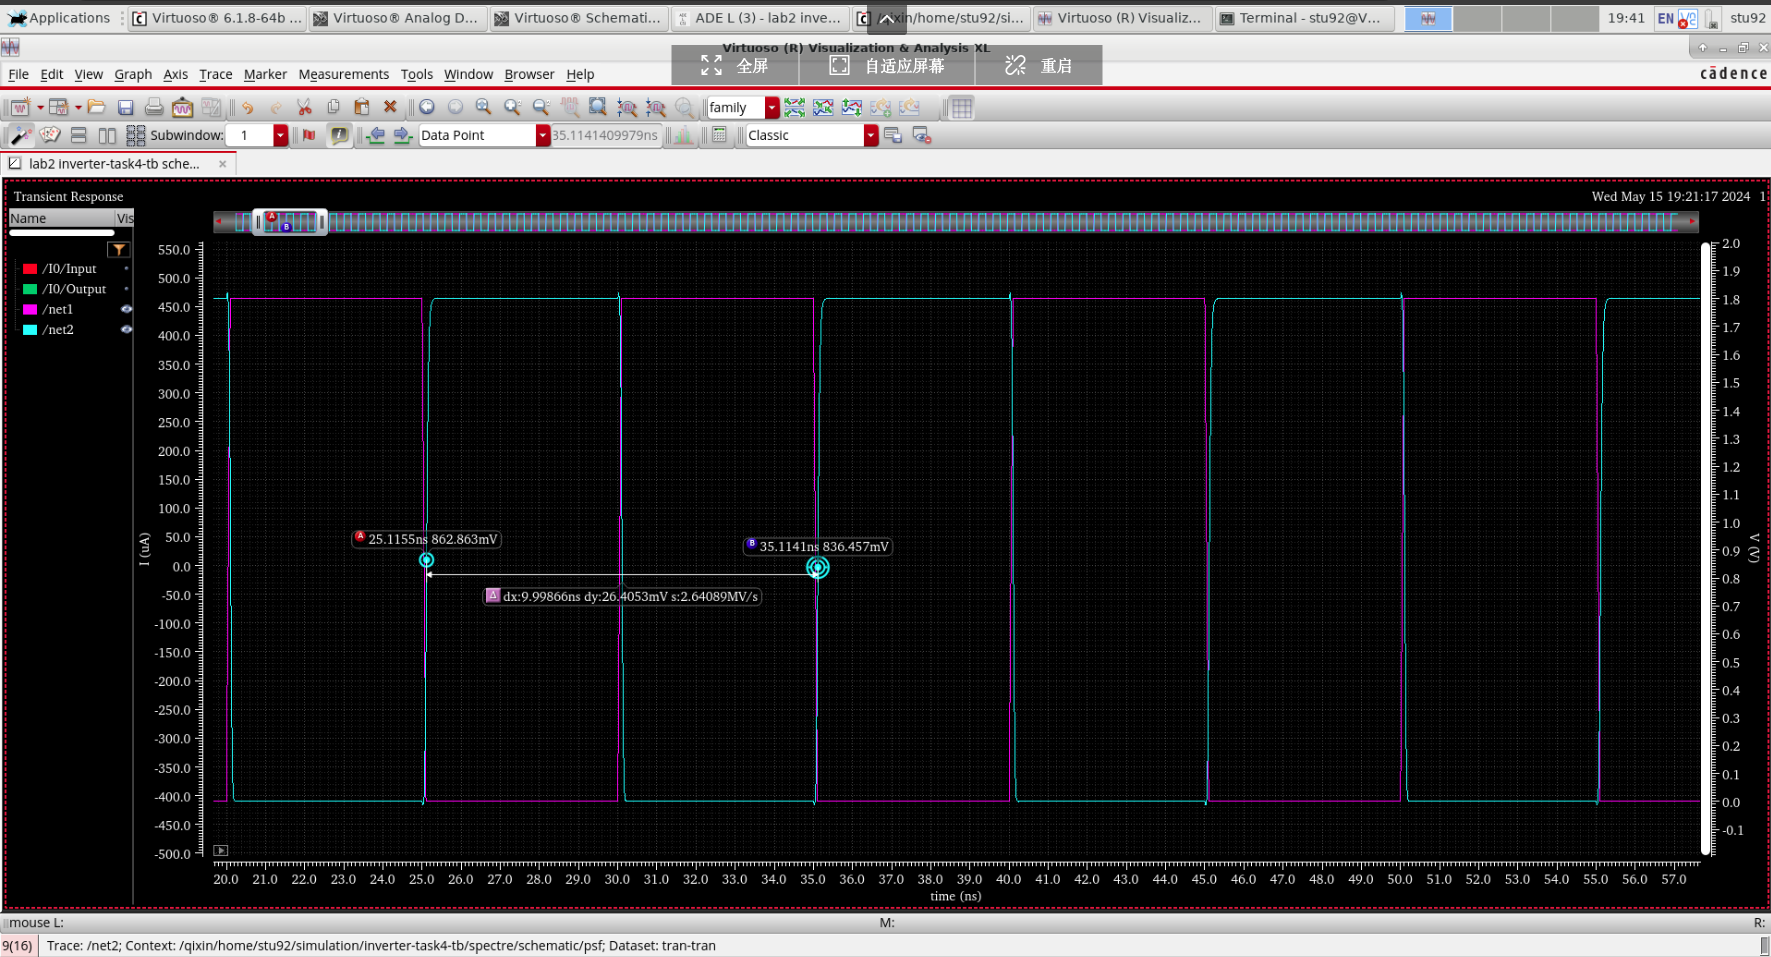
\includegraphics[width=0.8\textwidth]{task4/task4-inverter-tb-wave-5.png}
  \caption{Question 2}
\end{figure}

A点:25.1155ns 862.863mV
B点:35.1141ns 836.457mV

由A点和B点坐标计算得到周期为 9.9986ns

\section{实验总结和感悟}

通过本次实验,我学会了使用 Cadence 进行电路仿真分析,深入理解了 MOS 管和反相器的工作原理。在实验中,我学会了如何绘制 NMOS 管的 ID-VDS 特性曲线,如何改变温度参数,如何绘制 CMOS 反相器的直流(DC)仿真分析和瞬态特性(Tran)仿真分析。通过实验,我对 MOS 管和反相器的工作原理有了更深入的理解,对 Cadence 工具的使用也更加熟练。

\end{document}
